% ============================================================================
% JassCardEye -- CAS-Transferarbeit (HSLU Informatik)
% Build: cd doc && tectonic transferarbeit.tex (führt BibTeX selbst aus)
% ============================================================================
\documentclass[11pt,a4paper,parskip=half]{scrartcl}

\usepackage[T1]{fontenc}
\usepackage{lmodern}
\usepackage[nswissgerman]{babel}
\usepackage{csquotes}
\usepackage{graphicx}
\usepackage{booktabs}
\usepackage{tabularx}
\usepackage{array}
\newcolumntype{Y}{>{\raggedright\arraybackslash}X}
\usepackage{longtable}
\usepackage{xcolor}
\usepackage{microtype}
\usepackage{amsmath}
\usepackage{enumitem}
\usepackage{float}
\usepackage{caption}
\usepackage{tikz}
\usetikzlibrary{positioning,arrows.meta,shapes.geometric,fit,calc}
\usepackage[margin=2.5cm]{geometry}
\usepackage[hidelinks]{hyperref}
\hypersetup{
  pdftitle={JassCardEye: Erkennung der obersten Jasskarte auf einem Kartenstapel mit YOLO und synthetischen Trainingsdaten},
  pdfauthor={Raphael Bolliger},
}

\graphicspath{{figures/}}
\captionsetup{font=small,labelfont=bf}
\setlist{nosep}
\setcounter{tocdepth}{2}

% Angaben, die nur der Autor kennt.

% Kurzschreibweisen
\newcommand{\map}[1]{mAP@#1}
\newcommand{\code}[1]{\texttt{#1}}

% TikZ-Stile für die Diagramme
\tikzset{
  box/.style={draw=black!70, rounded corners=2pt, align=center, font=\small,
              inner sep=5pt, minimum height=9mm, fill=white},
  data/.style={box, fill=blue!6},
  tool/.style={box, fill=orange!8},
  ext/.style={box, fill=black!4, draw=black!40},
  arrow/.style={-{Latex[length=2.2mm]}, thick, black!70},
  lbl/.style={font=\scriptsize, text=black!70, align=center},
}

\begin{document}

% Seite 1. Nach der HSLU-Vorlage frei gestaltbar; die Pflichtangaben stehen auf Seite 2.
\begin{titlepage}
  \centering
  \vspace*{1.5cm}

  {\large Hochschule Luzern -- Informatik\par}
  \vspace{2cm}

  {\Large\bfseries Erkennung der obersten Jasskarte auf einem Kartenstapel\\
   mit YOLO und synthetischen Trainingsdaten\par}
  \vspace{0.8cm}
  {\large Transferarbeit\par}

  \vspace{1.2cm}
  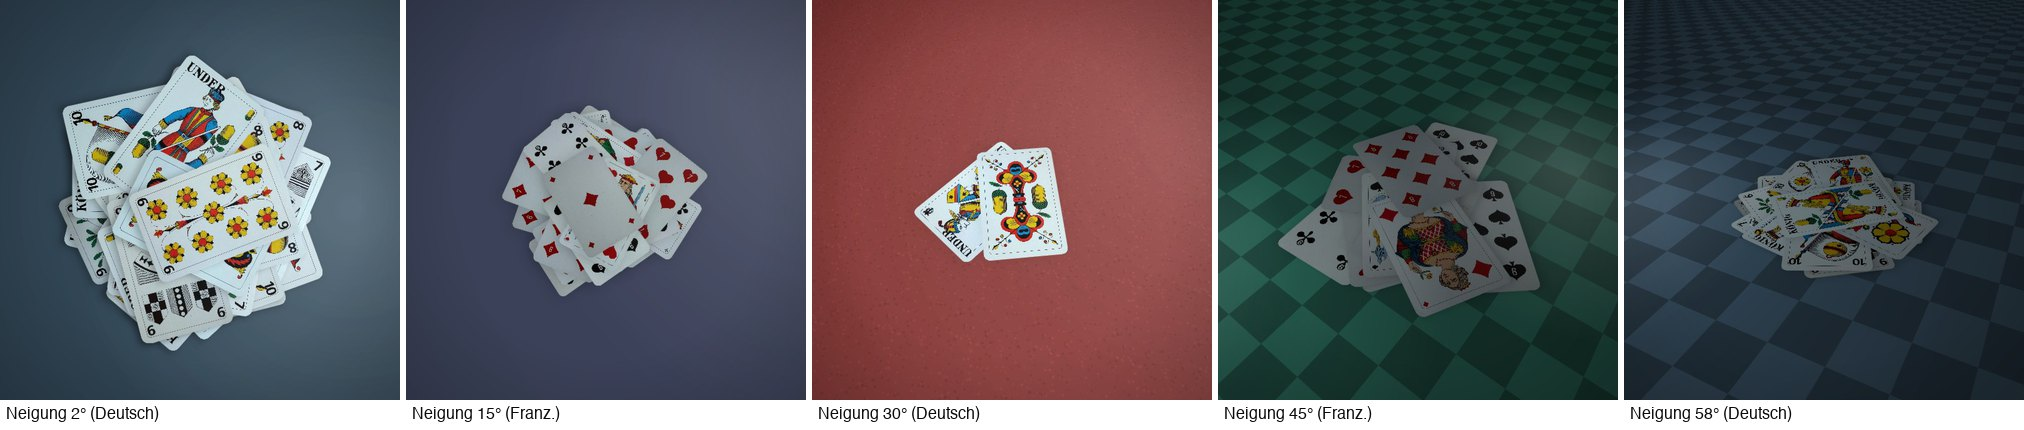
\includegraphics[width=0.7\textwidth]{synthetisch-winkel.jpg}\par
  \vspace{0.15cm}
  {\small Synthetisch erzeugte Trainingsbilder, Kameraneigung von 2\textdegree{} bis 58\textdegree{}\par}

  \vfill

  \begin{tabular}{ll}
    Autor:       & Raphael Bolliger \\
    Abgabedatum: & 20.09.2026 \\
    Repository:  & \url{https://github.com/yarx/JassCardEye} \\
  \end{tabular}

  \vspace{1cm}
\end{titlepage}

% Seite 2 nach der offiziellen HSLU-Vorlage (Vorlage_Deckblatt Transferarbeit.docx):
% Angaben zur Arbeit, Klassifizierung, Eidesstattliche Erklärung, ein Unterschriftenfeld.
{\large\bfseries Transferarbeit an der Hochschule Luzern -- Informatik\par}
\vspace{1.2em}

\noindent
\begin{tabular}{@{}p{4.0cm}p{11.6cm}@{}}
  Titel:                    & Erkennung der obersten Jasskarte auf einem Kartenstapel
                              mit YOLO und synthetischen Trainingsdaten \\[0.4em]
  Teilnehmer:               & Raphael Bolliger \\[0.4em]
  Programm:                 & CAS Machine Learning \\[0.4em]
  Zeitraum:                 & Juli bis September 2026 \\[0.4em]
  Programmleitung:          & Prof.\ Dr.\ Aygul Zagidullina / Prof.\ Dr.\ Umberto Michelucci \\[0.4em]
  Betreuung/Referat:        & Prof.\ Dr.\ Umberto Michelucci \\
\end{tabular}

\vspace{1.4em}
\noindent
Codierung / Klassifizierung der Arbeit:

\vspace{0.6em}
\noindent
\framebox[2.4ex]{\rule[-0.25ex]{0pt}{1.9ex}X}\quad Öffentlich (Normalfall)\\[0.4em]
\framebox[2.4ex]{\rule[-0.25ex]{0pt}{1.9ex}\phantom{X}}\quad Vertraulich

\vspace{2em}
{\large\bfseries Eidesstattliche Erklärung\par}
\vspace{0.8em}

\noindent
Ich erkläre hiermit, dass ich die vorliegende Arbeit selbständig und ohne
unerlaubte fremde Hilfe angefertigt habe. Alle verwendeten Quellen, Literatur
und Hilfsmittel (insbesondere künstliche Intelligenz oder sonstige verwendete
Instrumente) wurden urheberrechts- und datenschutzkonform verwendet und
wörtlich oder inhaltlich entnommene Stellen als solche kenntlich gemacht. Das
Vertraulichkeitsinteresse des Auftraggebers wurde gewahrt und die
Urheberrechtsbestimmungen der Hochschule Luzern respektiert.

\vspace{0.8em}
\noindent
Ich nehme zur Kenntnis, dass meine verfassten Arbeiten mit elektronischen
Hilfsmitteln auf Plagiate überprüft werden können. Ich bin bei begründetem
Verdacht auf eine unerlaubte oder nicht gekennzeichnete Anwendung auf Einladung
hin verpflichtet, an der Klärung des Verdachts mitzuwirken, z.\,B. durch
Teilnahme an einem Gespräch.

\vspace{0.8em}
\noindent
Der Einsatz von künstlicher Intelligenz in dieser Arbeit ist in
Anhang~\ref{app:ki-deklaration} deklariert.

\vspace{3em}
\noindent
Ort / Datum, Unterschrift\quad\rule{9cm}{0.4pt}

\vspace{2em}
\noindent
{\small\itshape Geistiges Eigentum gemäss der Studienordnung für die Ausbildung
an der Hochschule Luzern, FH Zentralschweiz\par}

\clearpage

\section*{Zusammenfassung}
\addcontentsline{toc}{section}{Zusammenfassung}

Beim Jassen werden die Karten am Ende einer Runde von Hand gezählt. Das
kostet Zeit und ist besonders für ungeübte Spielende mühsam. Ziel dieser
Arbeit ist ein Modell, das in einem Videostream die oberste Karte eines
Stapels in Echtzeit erkennt und so das Zählen mit dem Smartphone ermöglicht.

Das Training erfolgt ausschliesslich mit synthetisch erzeugten Bildern. Ein
Generator setzt aus 72 fotografierten Jasskarten Stapel mit unterschiedlichen
Kameraperspektiven, Beleuchtungen und Tischoberflächen zusammen und erzeugt
die Labels automatisch. Drei Ansätze auf Basis von YOLO11 werden verglichen:

\begin{itemize}
  \item Variante~A klassifiziert das gesamte Bild.
  \item Variante~B lokalisiert zuerst die oberste Karte und klassifiziert
    anschliessend ihren entzerrten Ausschnitt.
  \item Variante~C erkennt Klasse und Position der obersten Karte mit einer
    achsenparallelen Bounding Box in einem Schritt.
\end{itemize}

Geprüft werden die Modelle auf eigenen, von Hand gelabelten realen Aufnahmen.
Die letzte Datenmengenreihe vergleicht sechs Bildanzahlen auf demselben
Validierungsset mit 813 Frames. Variante~C verbessert sich mit mehr
Trainingsbildern und erreicht bei 200'000 Bildern eine \map{50} von 0.908.
Ein zusätzlicher Lauf mit 500'000 Bildern bringt keinen weiteren Gewinn.
Sie liefert Klasse und Position mit einem Modell und läuft in den Apps
in Echtzeit. Variante~A liefert keine Position. Bei Variante~B ist die
gesamte zweistufige Erkennung auf diesem Stand nicht verlässlich gemessen.

Dies aufgrund der bereits in der ersten Stufe von Variante~B schlechteren Ergebnisse gegenüber C, daraus würden auch für die Stufe B2 keine Verbsserungen erfolgen.

Die Ergebnisse sprechen deshalb am stärksten für Variante~C.

Das Modell wurde in eine iPhone- und eine Android-App zur Kartenzählung
integriert. Fehlvorhersagen, insbesondere bei Karten im Wurf, bleiben eine
Herausforderung. Eine Stabilitätsregel kann kurze Fehlerfolgen abfangen,
behebt aber nicht alle Fehlalarme. Da viele Validierungsbilder aus denselben
Videos stammen und ein unabhängiges Testset fehlt, sind die gemessenen
Trefferquoten vorsichtig einzuordnen.


Das Training läuft automatisiert auf
zeitweise gemieteten Cloud-GPUs und ist über Commit, Seed und Konfiguration
nachvollziehbar.

\clearpage


{\small\tableofcontents}
\clearpage
\listoffigures
\listoftables
\clearpage

\section{Einleitung}\label{sec:einleitung}

\subsection{Ausgangslage}\label{sec:ausgangslage}

Jass ist ein verbreitetes Kartenspiel in der Schweiz. Am Ende einer Runde
werden die gewonnenen Stiche einer Partei gezählt, indem die Karten
nacheinander abgelegt und ihre Punktwerte addiert werden. Das kostet Zeit
und ist besonders für ungeübte Spielende fehleranfällig.

Smartphones haben heute leistungsfähige Kameras und Recheneinheiten für
maschinelles Lernen. Damit lässt sich ein Kartenstapel direkt am Spieltisch
filmen und auswerten, ohne einen Server zu benötigen. In dieser Arbeit wird
ein Modell trainiert, das in einem Videostream jeweils die oberste Karte
eines Stapels erkennt. Die App soll daraus die Punkte der Runde berechnen.

Ursprünglich war vorgesehen, die Trainingsbilder selbst zu fotografieren
und von Hand zu labeln. Für die benötigte Menge erwies sich das früh als
unrealistisch. Deshalb werden die Trainingsbilder synthetisch aus Fotos der
einzelnen Karten erzeugt. Diese Kurskorrektur ist ein wichtiger Teil der
Arbeit und wird in Abschnitt~\ref{sec:verworfen} reflektiert.

\subsection{Problemstellung}\label{sec:problemstellung}

Erkannt werden soll nur die oberste Karte eines Stapels überlappender
Karten. Darunterliegende, teilweise sichtbare Karten dürfen nicht gezählt
werden. Die Erkennung muss zuverlässig und schnell genug sein, damit die
App in einer realen Spielsituation genutzt werden kann. Wer die Karten
zählt, soll das Ergebnis nicht nach jeder Erkennung selbst kontrollieren
müssen.

Die Aufnahmebedingungen variieren: Die Kamera wird von Hand geführt, der
Abstand und der Winkel ändern sich, und das Licht kann von einer
Deckenlampe, vom Tageslicht oder von der Taschenlampe des Smartphones
kommen. Auch die Unterlage wechselt zwischen Jassteppich, Holz und Stein.
In vielen Frames ist keine eindeutig lesbare oberste Karte zu sehen, etwa
wenn eine Karte geworfen wird, verwischt oder den Stapel verdeckt.

Für solche Situationen gilt die Prämisse dieser Arbeit: \emph{Lieber
nichts als falsch.} Eine übersehene Karte kann erneut vor die Kamera
gehalten werden. Eine falsch gezählte Karte bleibt dagegen möglicherweise
unbemerkt und verfälscht das Resultat. Gerade weil ein Videostream mehrere
Frames derselben Karte liefert, kann die App kurze Lücken überbrücken.

Der Engpass liegt bei den Trainingsdaten. Ultralytics nennt 1500 Bilder je
Klasse als Richtwert für eigene Datensätze \cite{ultralytics2025tips}.
Schon für die 36 Karten eines Blatts wären das 54'000 Bilder. Diese Menge
von Kartenstapeln lässt sich im Rahmen der Transferarbeit weder sinnvoll
fotografieren noch von Hand labeln.

\subsection{Ziele und Forschungsfragen}\label{sec:ziele}

Ziel ist ein mobiler Prototyp, der die oberste Karte mithilfe eines auf
synthetischen Bildern trainierten Modells erkennt und die Jasspunkte eines
Stapels zählt. Daraus ergeben sich zwei Forschungsfragen:

\begin{description}
  \item[FF1] Welcher Erkennungsansatz (einstufiger Detektor, zweistufige
    Erkennung mit orientierter Box und Klassifikation oder reine
    Bildklassifikation) bietet auf dem Smartphone die beste Balance
    zwischen Genauigkeit und Rechenaufwand?
  \item[FF2] Wie gut übertragen sich Modelle, die ausschliesslich auf
    synthetisch erzeugten Bildern trainiert wurden, auf reale Fotos?
\end{description}

Die ursprüngliche Themeneingabe sah auch einen Vergleich zwischen realen
und synthetischen Trainingsbildern vor. Da keine ausreichend grosse Menge
realer Trainingsbilder erstellt werden konnte, wird stattdessen der
Transfer von synthetischen Trainingsbildern auf reale Aufnahmen geprüft.
Ebenso entfiel der vorgesehene Vergleich verschiedener Modellgrössen.
Alle Modelle verwenden die kleinste Grösse n, weil sie auf dem Smartphone
in Echtzeit läuft. An die Stelle dieses Vergleichs trat der Vergleich der
drei Erkennungsansätze. Geschwindigkeit und Modellgrösse wurden für den
gewählten Ansatz auf vier Geräten gemessen
(Abschnitt~\ref{sec:app}).

\subsection{Abgrenzung}\label{sec:abgrenzung}

Die App erkennt die oberste Karte und zählt den Stapel einer Partei, in der
Praxis häufig den kleineren der beiden Stapel. Aus der Gesamtpunktzahl
der Karten und der Angabe zum letzten Stich berechnet sie auch die Punkte
der anderen Partei. Ein vollständiges Scoring mit Weis und Stöck ist
nicht Teil der Arbeit.

Die Karten liegen flach auf dem Tisch. Gekippte oder stehende Karten sowie
Hände im Bild werden im Generator nicht modelliert. Unterstützt werden
zwei Blätter mit je 36 Karten: ein französisches Standardblatt von
AGMüller und das deutschschweizerische Blatt \enquote{Schaffhauser
Spielkarten Opti-Quatro} desselben Herstellers.

Wie gut das Modell leicht abweichende Kartendesigns oder Sondereditionen
erkennt, wurde nicht untersucht. Diese Grenze wird in
Abschnitt~\ref{sec:grenzen} erläutert.

\section{Grundlagen und Stand der Technik}\label{sec:grundlagen}

\subsection{Jass und Jasskarten}\label{sec:jass}

Ein Jassblatt hat 36 Karten in vier Farben mit je neun Werten.
Diese Arbeit verwendet zwei Blätter von AGMüller: ein französisches
Standardblatt und das deutschschweizerische \enquote{Schaffhauser
Spielkarten Opti-Quatro}. Eine Partie wird mit einem Blatt gespielt; die
beiden werden nicht gemischt. Viele Karten sehen nach einer Drehung um
180\textdegree{} fast gleich aus. Spiegeln verändert dagegen die Anordnung
der Eckzeichen und eignet sich deshalb nicht als Augmentierung.

Wie viele Punkte eine Karte zählt, hängt von der Spielart und von der
Trumpffarbe ab. Bei den Spielarten, welche die App unterstützt, ergeben
alle Karten zusammen 152 Punkte. Für den letzten Stich kommen weitere
5 Punkte hinzu \cite{swisslos2026grundlagen}. Bei anderen Spielarten
können auch bestimmte Stiche oder Kartenkombinationen zusätzliche Punkte
geben. In dieser Arbeit stehen die Erkennung der obersten Karte und die
Berechnung der Punkte eines Stapels im Mittelpunkt.

\subsection{Objekterkennung mit Deep Learning}\label{sec:objekterkennung}

Bildklassifikation ordnet einem Bild eine Klasse zu. Objektdetektion gibt
zusätzlich die Position als Bounding Box an. Einstufige Detektoren wie YOLO
sagen Box und Klasse in einem Durchgang voraus \cite{redmon2016yolo}. Ein
zweistufiger Ansatz lokalisiert zuerst und klassifiziert danach. In dieser
Arbeit werden beide Ansätze und die reine Klassifikation verglichen
(Abschnitt~\ref{sec:varianten}).

\subsection{Die YOLO-Familie und YOLO11}\label{sec:yolo}

Verwendet wird YOLO11 mit Ultralytics \cite{jocher2024ultralytics,
ultralytics2025yolo11docs,khanam2024yolov11}. Für die drei Ansätze werden verschiedene
Ausführungen derselben Modellfamilie trainiert: A und B$_2$ klassifizieren,
B$_1$ lokalisiert mit einer gedrehten Box, und C liefert eine
achsenparallele Box samt Kartenklasse. Alle nutzen die kleinste
Modellgrösse n, damit sie auf einem Smartphone laufen. Die
Mosaic-Augmentierung setzt beim Training vier Bilder zusammen und wird
in den letzten Epochen abgeschaltet \cite{bochkovskiy2020yolov4,ultralytics2025augment}.

YOLO26 erschien erst im Januar 2026 und war damit zu Beginn der
Umsetzung noch sehr neu. Das Modell kann Vorhersagen ohne
nachgelagerte Non-Maximum Suppression ausgeben. Dadurch unterscheidet
sich sein Ausgabeformat von YOLO11 \cite{ultralytics2026yolo26}. Die
Unterstützung dieses Formats war in mobilen Anwendungen zu diesem
Zeitpunkt noch nicht vollständig ausgereift. Ein GitHub-Issue vom
Mai 2026 zeigt beispielsweise, dass die Verarbeitung dieser Ausgabe
noch ergänzt werden musste \cite{ultralytics2026flutter487}.

Für diese Arbeit war eine verlässliche Integration auf iOS und Android
wichtiger als der Einsatz der neuesten Modellversion. YOLO11 liess sich
bereits stabil trainieren, exportieren und in beiden Apps ausführen.
Deshalb wurde das Projekt mit YOLO11 ausgeführt.

\subsection{Metriken}\label{sec:metriken}

Die Modelle werden mit verschiedenen Kennzahlen verglichen. Bei einem
Detektor zählt neben der richtigen Kartenklasse auch die Position. Die
\emph{Intersection over Union} (IoU) misst, wie stark sich die
vorhergesagte Box und die von Hand gesetzte Box überlappen: 0 bedeutet
keine Überlappung, 1 eine deckungsgleiche Box.

Die \emph{Precision} gibt an, wie viele der gemeldeten Karten richtig
sind. Meldet ein Modell zehn Karten und acht davon sind richtig, beträgt
die Precision 80\,\%. Der \emph{Recall} beschreibt, wie viele der
vorhandenen Karten gefunden werden. Sind zehn Karten vorhanden und das
Modell findet acht davon, beträgt der Recall ebenfalls 80\,\%. Beide
Werte hängen von der gewählten Konfidenzschwelle ab.

Die \emph{Average Precision} (AP) fasst Precision und Recall für eine
Kartenklasse zusammen. Die \emph{mean Average Precision} (mAP) bildet
daraus den Mittelwert über alle Klassen. Bei \map{50} zählt eine
Vorhersage nur dann als richtig, wenn sie mindestens eine IoU von 0.5
erreicht \cite{everingham2010pascal}. \map{50--95} verwendet mehrere
IoU-Schwellen zwischen 0.5 und 0.95. Ungenaue Boxen werden dadurch
strenger bewertet
\cite{lin2014coco,coco2015eval,ultralytics2025metrics}. Die mAP ist
deshalb nicht mit dem Anteil korrekt benannter oberster Karten
gleichzusetzen.

Für die reine Bildklassifikation wird die \emph{Top-1-Genauigkeit}
verwendet: Der Klassenname mit dem höchsten Wert muss stimmen. Für die
App ist zusätzlich die einfachere Zahl \enquote{oberste Karte richtig}
wichtig. Sie gibt an, auf wie vielen realen Fotos das Modell die oberste
Karte korrekt benennt. Ob die App sie tatsächlich zählt, hängt
anschliessend noch von
Konfidenzschwelle und Stabilitätsregel ab
(Abschnitt~\ref{sec:betriebspunkt}).

\subsection{Transfer Learning}\label{sec:transfer}

Alle Ansätze starten mit vortrainierten YOLO11n-Gewichten, statt ein Netz
von Grund auf zu trainieren \cite{pan2010transfer}. Die Startgewichte
von C stammen aus dem Training auf COCO-Alltagsbildern \cite{lin2014coco}, jene von B$_1$
aus DOTA-Luftbildern \cite{xia2018dota} und jene der Klassifikatoren A und B$_2$ aus
ImageNet \cite{russakovsky2015imagenet,ultralytics2025yolo11docs}. So können bereits gelernte
Bildmerkmale übernommen werden. Die Ausgabe wird für die
projektspezifischen Kartenklassen neu trainiert; deren Anzahl ist je
Ansatz verschieden (Abschnitt~\ref{sec:varianten}).

\subsection{Synthetische Trainingsdaten und Domain Randomization}\label{sec:synthdata}

Gerenderte Bilder haben den Vorteil, dass ihre Labels automatisch und
genau erzeugt werden können. Die Herausforderung liegt bei der
Übertragung auf reale Fotos. Dieser Unterschied wird als
Sim-to-Real-Gap bezeichnet.

Domain Randomization soll diese Lücke verkleinern. Dabei werden
Perspektive, Licht, Textur und Kameraeinstellungen bewusst verändert.
Das Modell sieht dadurch viele unterschiedliche Situationen und soll
lernen, welche Merkmale auch auf realen Bildern wichtig sind
\cite{tobin2017domain}. Dafür muss nicht jedes gerenderte Bild möglichst
echt aussehen. Auch einfache synthetische Bilder können für das Training
geeignet sein, wenn die Objekte plausibel in die Szene eingefügt werden
\cite{dwibedi2017cut}.

Tremblay et al. trainierten einen Detektor nur mit synthetischen Bildern
und konnten damit Autos auf realen Aufnahmen erkennen. Wenige zusätzliche
reale Trainingsbilder verbesserten das Ergebnis weiter
\cite{tremblay2018training}. Ein ähnlicher Ansatz wurde bereits für
Spielkarten verwendet. Das Projekt von geaxgx erzeugt aus fotografierten
Pokerkarten einen synthetischen Datensatz und trainiert damit YOLOv3.
Erkannt werden dort die Eckzeichen der Karten. Eine Auswertung auf realen
Fotos wird jedoch nicht ausgewiesen \cite{geaxgx2018cards}.

Ultralytics empfiehlt mindestens 1500 Bilder je Klasse
\cite{ultralytics2025tips}. Bereits für ein Blatt mit 36 Karten ist diese
Menge von Hand kaum zu erstellen und zu labeln. In dieser Arbeit werden
die Trainingsbilder deshalb gerendert. Die Prüfung erfolgt auf eigenen
realen Aufnahmen (Abschnitt~\ref{sec:validierung}).

\subsection{On-Device-Inferenz}\label{sec:ondevice}

Core ML und Vision führen das exportierte Modell auf iOS aus
\cite{apple2025coreml,apple2025vision}. Auf Android übernimmt LiteRT diese
Aufgabe \cite{google2026litert}. Die beiden Exporte stammen aus denselben Gewichten. Die
Laufzeiten unterscheiden sich bei der Verarbeitung der Boxen und
Konfidenzen, was für den Vergleich der App-Ausgaben geprüft werden muss
(Abschnitt~\ref{sec:betriebspunkt}).

\section{Lösungskonzept und Methodik}\label{sec:methodik}

\subsection{Anforderungen}\label{sec:anforderungen}

Tabelle~\ref{tab:anforderungen} fasst die Anforderungen zusammen, die aus der
Problemstellung und der Themeneingabe abgeleitet wurden.

\begin{table}[H]
\centering\small
\begin{tabularx}{\textwidth}{@{}lY@{}}
\toprule
\textbf{Bereich} & \textbf{Anforderung} \\
\midrule
Erkennung & Die App erkennt Klasse und Position der obersten Karte bei wechselndem Winkel, Abstand, Licht und Hintergrund. Auf Frames ohne gültige Karte darf sie nichts erkennen. Eine falsch gezählte Karte wiegt schwerer als eine übersehene. \\
Latenz & Die Erkennung läuft direkt auf dem Gerät in Echtzeit. Das Ziel liegt unter 50\,ms pro Bild. \\
Daten & Aus wenigen Kartenscans lassen sich Trainingsbilder in beliebiger Menge erzeugen. Dieselbe Konfiguration liefert auf jeder Maschine bit-identische Bilder. \\
Vergleich & Drei Erkennungsansätze werden mit denselben Bildern trainiert und auf realen Aufnahmen verglichen. \\
Plattform & Datengenerierung und Training sollen möglichst unabhängig vom Betriebssystem laufen. Cloud-Anbieter und Speicherlösungen müssen austauschbar bleiben, damit das Projekt nicht an eine Plattform gebunden ist. \\
App & Die App erkennt Karten live über die Kamera und zählt ihre Punkte nach den Jass-Regeln. iOS und Android verwenden dasselbe Modell. \\
Nachvollziehbarkeit & Jeder Trainingslauf lässt sich auf Commit, Seed und Bildanzahl zurückführen. Für jedes in einer App enthaltene Modell ist der zugehörige Lauf dokumentiert. \\
\bottomrule
\end{tabularx}
\caption{Anforderungen an das System.}
\label{tab:anforderungen}
\end{table}

\subsection{Systemarchitektur}\label{sec:architektur}

Das System besteht aus einer .NET-10-Lösung für Datenerzeugung und
Sichtkontrolle, Python-Skripten für Training und Export sowie zwei Apps.
Abbildung~\ref{fig:architektur} zeigt den Weg vom Kartenscan bis zur App.

\begin{figure}[H]
\centering
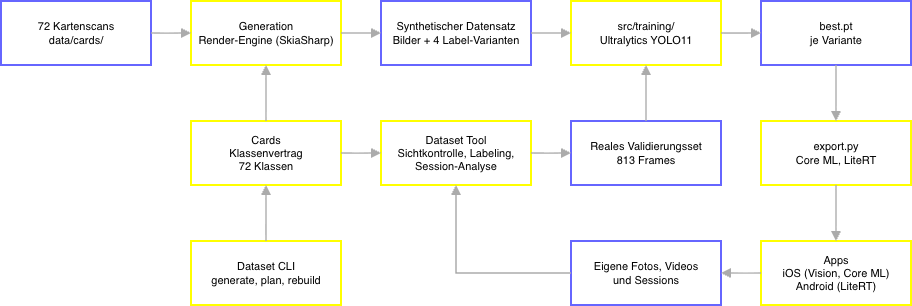
\includegraphics[width=\textwidth]{systemarchitecture.drawio.png}
\caption{Systemarchitektur und Datenfluss. Gelb hinterlegt sind eigene Werkzeuge, blau die Daten.}
\label{fig:architektur}
\end{figure}

Das Projekt \code{Cards} legt die 72 Klassen und ihre IDs fest:
$\mathrm{ID}=9\cdot\mathrm{Farbe}+\mathrm{Wert}$. Das französische Blatt
belegt die IDs 0--35, das deutsche Blatt die IDs 36--71. Datengenerator,
Training und Apps verwenden diese Zuordnung. \code{Generation} rendert
die Bilder mit SkiaSharp \cite{skiasharp2025}. Die \code{Dataset CLI}
startet die Erzeugung, zeigt den geplanten Winkel- und Blattverlauf an
und stellt abgeleitete Datensatzteile wieder her. Das Dataset Tool dient
zur Sichtkontrolle, zum Labeln realer Fotos und zur Analyse
aufgezeichneter Sessions. Das Training verwendet Ultralytics und
PyTorch \cite{paszke2019pytorch}.

\subsection{Variantenbildung: drei Erkennungsansätze}\label{sec:varianten}

Verglichen werden drei Ansätze, die sich darin unterscheiden, ob und wie
sie die oberste Karte lokalisieren (Abbildung~\ref{fig:varianten}). Alle
müssen für den Einsatz auf dem Smartphone schnell genug sein.

\begin{figure}[H]
\centering
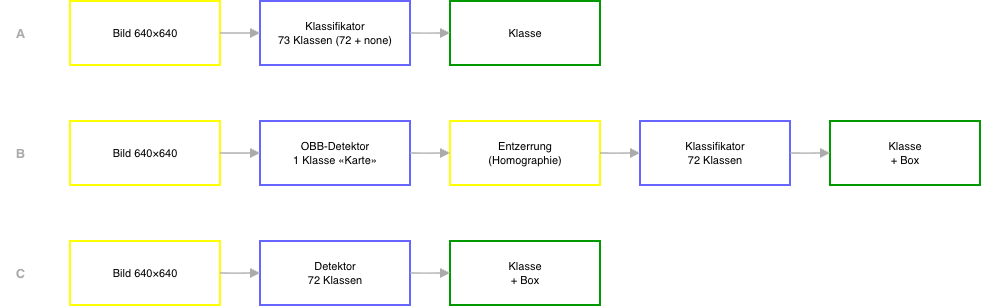
\includegraphics[width=\textwidth]{erkennungsvarianten.drawio.png}
\caption{Die drei Erkennungsansätze. A klassifiziert das ganze Bild, B lokalisiert die Karte mit einer orientierten Box und klassifiziert den entzerrten Ausschnitt, C erkennt Box und Klasse in einem Schritt.}
\label{fig:varianten}
\end{figure}

A klassifiziert das ganze Bild in 72 Kartenklassen und die Klasse
\code{none}, liefert aber keine Position. B findet zuerst die vier Ecken
der obersten Karte mit einer orientierten Box. Der entzerrte Ausschnitt
wird danach separat klassifiziert. Das kostet Zeit. Fehler der ersten
Stufe wirken sich auf die zweite aus. C erkennt Klasse und
achsenparallele Box in einem Schritt. Alle drei Ansätze erhalten
dieselben gerenderten Bilder. Nur ihre Labels unterscheiden sich. So
werden die Ansätze auf gleicher Datengrundlage verglichen. Für B wurde
eine orientierte Box gewählt, weil eine achsenparallele Box bei gedrehten
Karten viel Hintergrund im Ausschnitt lässt.

\subsection{Validierungsstrategie}\label{sec:validierung}

Trainiert wird ausschliesslich auf synthetischen Bildern, geprüft auf
selbst aufgenommenen realen Fotos. Der aktuelle Validierungsdatensatz
umfasst 813 Frames. Auf 513 ist eine Karte gelabelt, 300 sind Negative.
Die realen Aufnahmen stammen aus Videos, einer Fotoserie und
Negativfotos. Die Ergebnisvergleiche nennen jeweils den verwendeten
Validierungsstand. Die abschliessende Datenmengenreihe berichtet
\map{50} für die Detektoren C und B$_1$ sowie die Top-1-Genauigkeit
für die Klassifikatoren A und B$_2$. B$_2$ erhält dabei Ausschnitte
aus den von Hand gesetzten Ecken. Viele Frames stammen aus
denselben Videos und sind deshalb nicht unabhängig. Ein separates
Testset fehlt (Abschnitt~\ref{sec:grenzen}).

\subsection{Messaufbau und Unsicherheit}\label{sec:setup}

Für die abschliessenden Vergleiche wurden YOLO11n-Modelle mit
vortrainierten Gewichten, 640 Pixel Bildgrösse und 20 Epochen trainiert.
Das Trainingsrezept steht in Abschnitt~\ref{sec:rezept}. Seed,
Bildanzahl und Commit sind für die ausgewerteten Modelle dokumentiert.
Bei jeder Bildzahl werden alle vier Modelle mit denselben gerenderten
Bildern trainiert. Die Datenmengenreihe verwendet sechs Bildzahlen bei
gleichem Generatorstand, Seed und Trainingsplan. Die Modelle wurden
auf denselben 813 realen Frames ausgewertet. Werte aus unterschiedlichen
Validierungsständen werden nicht direkt verglichen. Trainiert wurde
auf einem MacBook Pro M4 Max sowie auf gemieteten NVIDIA A100 und H100 \cite{runpod2025gpu}.

Die Laufzeit der eingereichten Variante~C wurde auf vier Smartphones
gemessen (Tabelle~\ref{tab:geraete}). Die Datenmengenreihe enthält keinen gemeinsamen
Latenzvergleich aller Ansätze.

Jede ausgewertete Konfiguration wurde nur mit einem Trainings-Seed
trainiert. Es gibt daher kein Mass für die Streuung zwischen
Wiederholungen. Kleine Unterschiede in den Metriken werden nicht
als gesicherter Effekt gedeutet.

\subsection{Reproduzierbarkeit und kleiner Datenfussabdruck}\label{sec:repro}

Ein Datensatz wird durch den Code und die Quellbilder sowie Seed,
Bildanzahl und Generatorparameter bestimmt. Jedes Bild nutzt einen
eigenen Zufallsstrom aus Seed und Bildindex. Die Gesamtzahl legt
zusätzlich den Kamerawinkel und das Blatt jedes Bildes fest. Darum
sind kleinere Datensätze keine Ausschnitte grösserer Läufe. Mit
gleicher Konfiguration werden auf verschiedenen Maschinen
bit-identische Bilder erzeugt. Das wurde durch zweimaliges Rendern
und einen byteweisen Vergleich geprüft. Parallelisierung ändert das
Ergebnis nicht. Auf zwölf Kernen entstehen rund 120 Bilder pro
Sekunde.

Versioniert werden die 72 Kartenscans, die realen Validierungsframes
mit ihren Labels und die 25 Fotos für reale Negative. Der
synthetische Datensatz wird vor jedem Training aus diesen Quellen
neu erzeugt und muss nicht gespeichert oder zwischen Maschinen
übertragen werden. Ein Lauf ist über Commit, Seed, Bildanzahl und
Konfiguration nachvollziehbar. Für 200'000 Bilder dauert die
Generierung je nach Maschine 20 bis 65 Minuten.

Die CI prüft die Daten mit \code{check\_dataset.py} und
\code{check\_run\_plan.py}. Das erste Skript sucht widersprüchliche
Labels, falsche Klassenordner und angeschnittene gelabelte Karten.
Das zweite prüft die gleichmässige Winkelverteilung und die hälftige
Aufteilung der Bilder auf beide Blätter.

\subsection{Vorgehen und Werkzeuge}\label{sec:vorgehen}

Die Umsetzung erfolgte in aufeinanderfolgenden Iterationen. Für jede
Iteration gab der Verfasser Claude Code eine konkrete fachliche
Anweisung. Danach prüfte er den erzeugten Code, führte Tests aus und
kontrollierte die Ergebnisse an Bildern, Labels und in den Apps. Fehler,
unklare Annahmen und Abweichungen wurden in einem Review festgehalten.
Darauf folgte eine neue und genauer formulierte Anweisung. Der Verfasser
entschied jeweils, ob ein Ergebnis übernommen oder nochmals überarbeitet
wurde. Die fachlichen Entscheide und die Abnahme lagen damit bei ihm.
Der zeitliche Verlauf steht im separaten Arbeitsjournal.
Die Rolle der KI wird in Abschnitt~\ref{sec:ki-reflexion} reflektiert
und in Anhang~\ref{app:ki-deklaration} deklariert.

Die Continuous Integration baut die .NET-Lösung, erzeugt einen kleinen
Datensatz, rekonstruiert das Validierungsset, führt die Prüfskripte
aus und prüft die Wertungstabelle der App. Das eigentliche Training
läuft auf gemieteten GPUs (Abschnitt~\ref{sec:pipeline}).

\section{Datengrundlage und synthetische Generierung}\label{sec:daten}

Die ursprüngliche Planung sah rund 2000 fotografierte und von Hand gelabelte
Kartenhaufen vor. Erste Versuche mit dem Online-Dienst Roboflow zeigten
schnell, dass weder das Fotografieren noch das Labeln dieser Menge realistisch
war. 2000 Bilder entsprechen bei 36 Klassen rund 56 Bildern je Klasse, also
3.7\,\% der von Ultralytics empfohlenen Untergrenze von 1500 Bildern je Klasse
\cite{ultralytics2025tips}. Der Entscheid fiel deshalb, die Karten einmal
zu fotografieren und alle Haufen daraus zu rendern. Dieses Kapitel
stellt die Quellscans und die unabhängige reale Prüfbasis mit ihren Labelregeln vor,
danach den Generator und seine Datensatzvarianten.

\subsection{Quellmaterial: 72 Kartenscans}\label{sec:scans}

Beide Blätter wurden Karte für Karte mit dem iPhone fotografiert, perspektivisch
begradigt und auf ein einheitliches Format gebracht: 1710$\times$2670 Pixel,
JPEG mit Qualität 75, ohne Farbprofil und Metadaten.

Durch wechselnde Lichtverhältnisse, insbesondere Sonneneinstrahlung, wiesen
einige Scans Farbunterschiede auf. Sie wurden soweit möglich an die übrigen
Karten angeglichen, damit das Modell den Farbstich nicht als Merkmal einer
einzelnen Karte lernt. Weitere Korrekturen beschreibt
Abschnitt~\ref{sec:label-qa}.

\subsection{Reales Validierungsset und Labeling-Werkzeug}\label{sec:labeling}

Das aktuelle Validierungsset umfasst 813 eigene Aufnahmen: 305 Karten des
französischen Blatts, 208 des deutschen Blatts und 300 Negative. Sie stammen
aus sieben Videos und einer Fotoserie des französischen Blatts, sechs Videos
des deutschen Blatts sowie Fotos ohne Karte. Die Aufnahmen zeigen
unterschiedliche Unterlagen, Lichtverhältnisse und Blickwinkel
(Abbildung~\ref{fig:realval}). Viele Frames stammen aus denselben Videos
und sind deshalb nicht unabhängig. Trainiert wird ausschliesslich auf
synthetischen Bildern.

\begin{figure}[H]
\centering
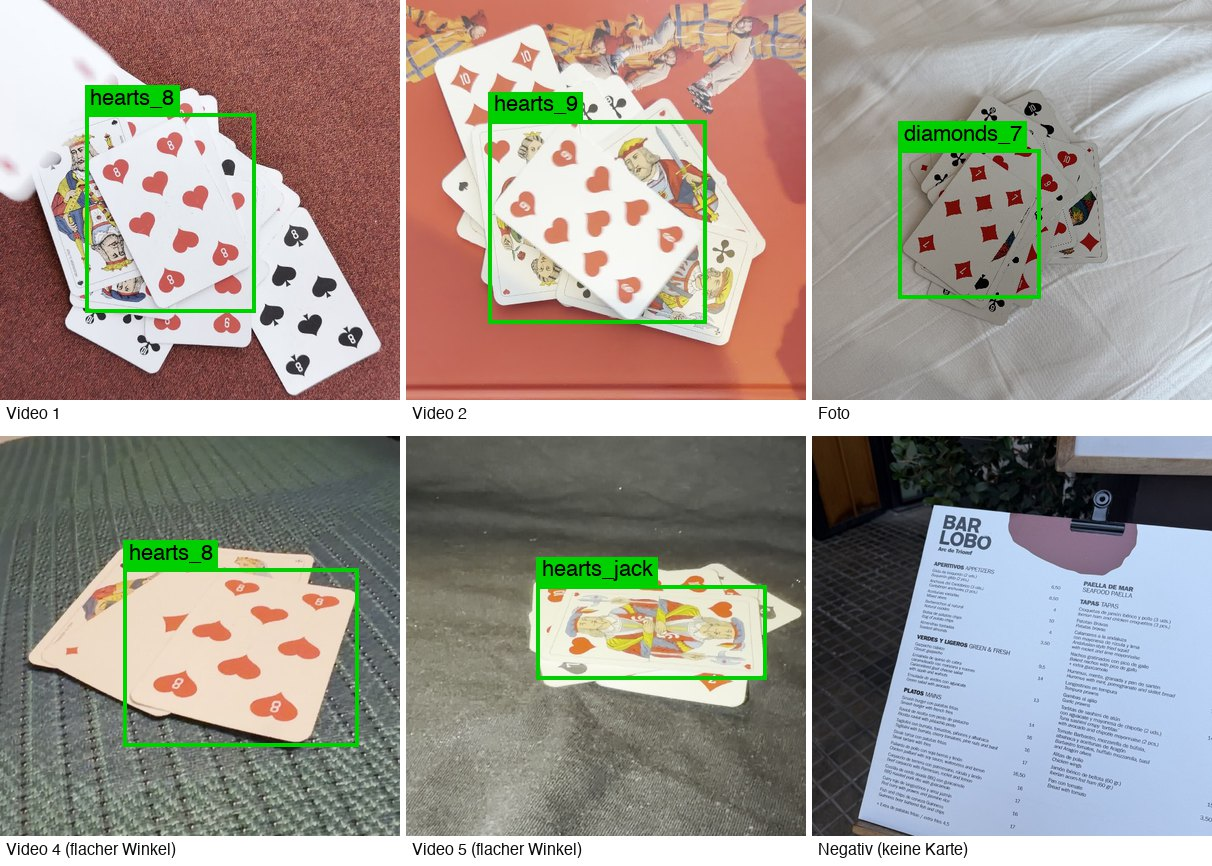
\includegraphics[width=0.85\textwidth]{real-val-beispiele.jpg}
\caption{Frames des realen Validierungssets mit ihren Labels: drei Aufnahmequellen, zwei flache Winkel und ein Negativ.}
\label{fig:realval}
\end{figure}

Das eigene Dataset Tool zeigt Bilder mit ihren Labels in allen Varianten.
Beim Labeln werden die vier Ecken der obersten Karte und ihre Klasse
gesetzt. Ein Frame ohne gültige Karte wird als \enquote{No card}
gespeichert. Aus einer Annotation entstehen alle vier Label-Formate.
Die Vorschau des entzerrten Ausschnitts zeigt, ob die Eckreihenfolge
stimmt (Abbildung~\ref{fig:dataset-tool-labeler}). Nicht quadratische
Fotos werden durch einen mittigen Ausschnitt auf 640$\times$640 gebracht.
Das entspricht dem Sucherquadrat der App. Das Werkzeug zerlegt Videos in
Frames und erlaubt Korrekturen an gespeicherten Labels. Die häufigen
Schritte lassen sich über die Tastatur bedienen.

\begin{figure}[H]
\centering
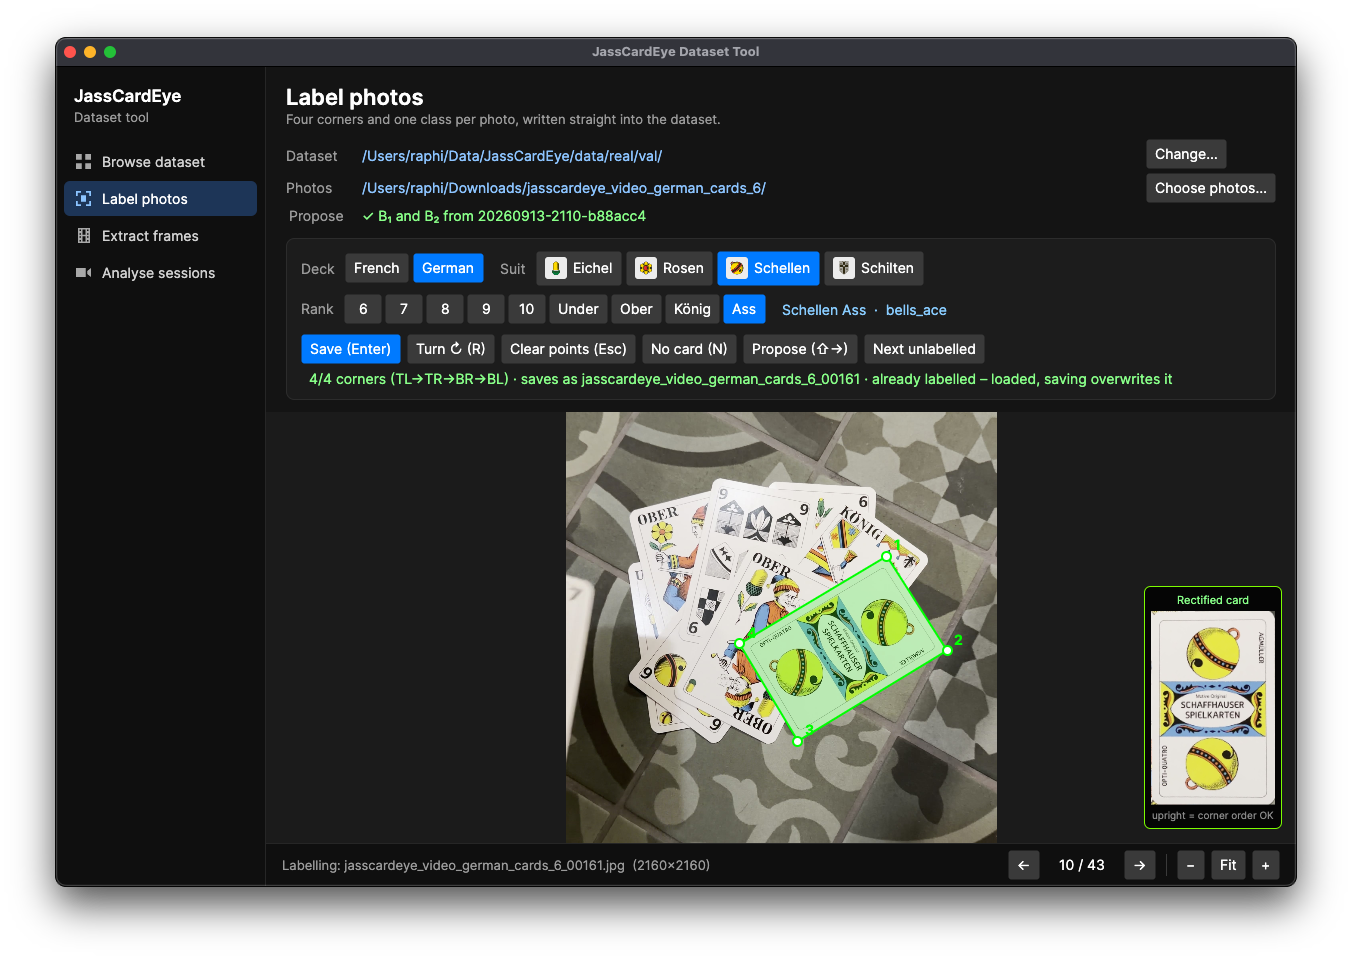
\includegraphics[width=0.9\textwidth]{dataset-tool-labeler.png}
\caption{Das eigene Dataset Tool beim Labeln eines realen Frames. Die vier Ecken markieren die oberste Karte. Rechts ist der entzerrte Ausschnitt zu sehen.}
\label{fig:dataset-tool-labeler}
\end{figure}

\subsection{Grenzfälle: was das Modell erkennen muss}\label{sec:grenzfaelle}

Die Grenze zwischen Karte und Negativ ist bei verwischten, teilweise
verdeckten oder sehr flach aufgenommenen Karten nicht immer eindeutig.
Für jedes reale Frame wurde entschieden, ob die oberste Karte lesbar ist.
Lesbare Karten wurden mit Klasse und Ecken gelabelt. Frames ohne lesbare
Karte wurden als \enquote{No card} gespeichert, unklare Fälle teilweise
ausgelassen. Das bleibt ein Problem für die Auswertung: Erkennt das Modell
eine Karte in einem als negativ gelabelten Frame, zählt dies als
Fehlalarm. Wird
eine schwierig lesbare, aber gelabelte Karte übersehen, zählt dies als
Fehler. Die Einteilung ist für das bestehende Set festgelegt. Ihre
Wirkung auf Fehlalarme muss mit weiteren Aufnahmen geprüft werden.
Eine eigene Markierung für schwierige Frames und eine getrennte
Auswertung sind noch nicht umgesetzt (Abschnitt~\ref{sec:ausblick}).

\subsection{Synthetische Szenen}\label{sec:szenen}

Eine Szene wird in drei Ebenen von hinten nach vorn aufgebaut. Zuunterst
liegt der \emph{Tischhintergrund}: ein prozedural erzeugtes, gleichmässig
wiederholtes Muster (Uni, Filz, Sprenkel, Karo, Tartan) in zufälliger Farbe.
Es liegt als Textur auf der Tischebene und wird mit derselben Kamera
projiziert wie die Karten, damit Fluchtpunkt und Perspektive übereinstimmen.
Darauf werden 0 bis 35 \emph{Unterkarten} aus dem Rest desselben Blatts
um die Mitte gestreut und gedreht. Zuoberst liegt die \emph{oberste Karte},
die allein gelabelt wird. Ihre Position variiert, damit ein Klassifikator
nicht \enquote{Mitte gleich Antwort} lernt.

Die Kamera ist eine Lochkamera, die aus einer zufälligen Position über dem
Tisch auf einen Punkt nahe der Mitte blickt. Für jede Karte werden die vier
Weltecken projiziert und der Kartenscan per Homographie exakt in das
projizierte Viereck verzerrt \cite{opencv2025calib3d}. Die Kameradistanz
variiert, die Neigung reicht von 0\textdegree{} bis 60\textdegree{} und
die Belichtung schwankt um $\pm$20\,\%. Jede Karte liegt 0.3\,mm höher als
die darunterliegende. Bei einem vollen Blatt wird der Stapel dadurch
rund einen Zentimeter hoch. Die abgerundeten Kartenecken bleiben
transparent und folgen der Perspektive.

In rund 65\,\% der Szenen beleuchtet eine Lampe den Tisch. Die übrigen
zeigen diffuses Raum- oder Tageslicht. Ein Teil der Lampenszenen erhält
eine zweite, aufhellende Lichtquelle. Das Lichtzentrum kann auch neben
oder hinter dem Haufen liegen. Die Karten werfen weiche Kontaktschatten,
und eine Vignette dunkelt die Bildecken ab. Abbildung~\ref{fig:synthetisch}
zeigt zwölf Beispiele.

\begin{figure}[H]
\centering
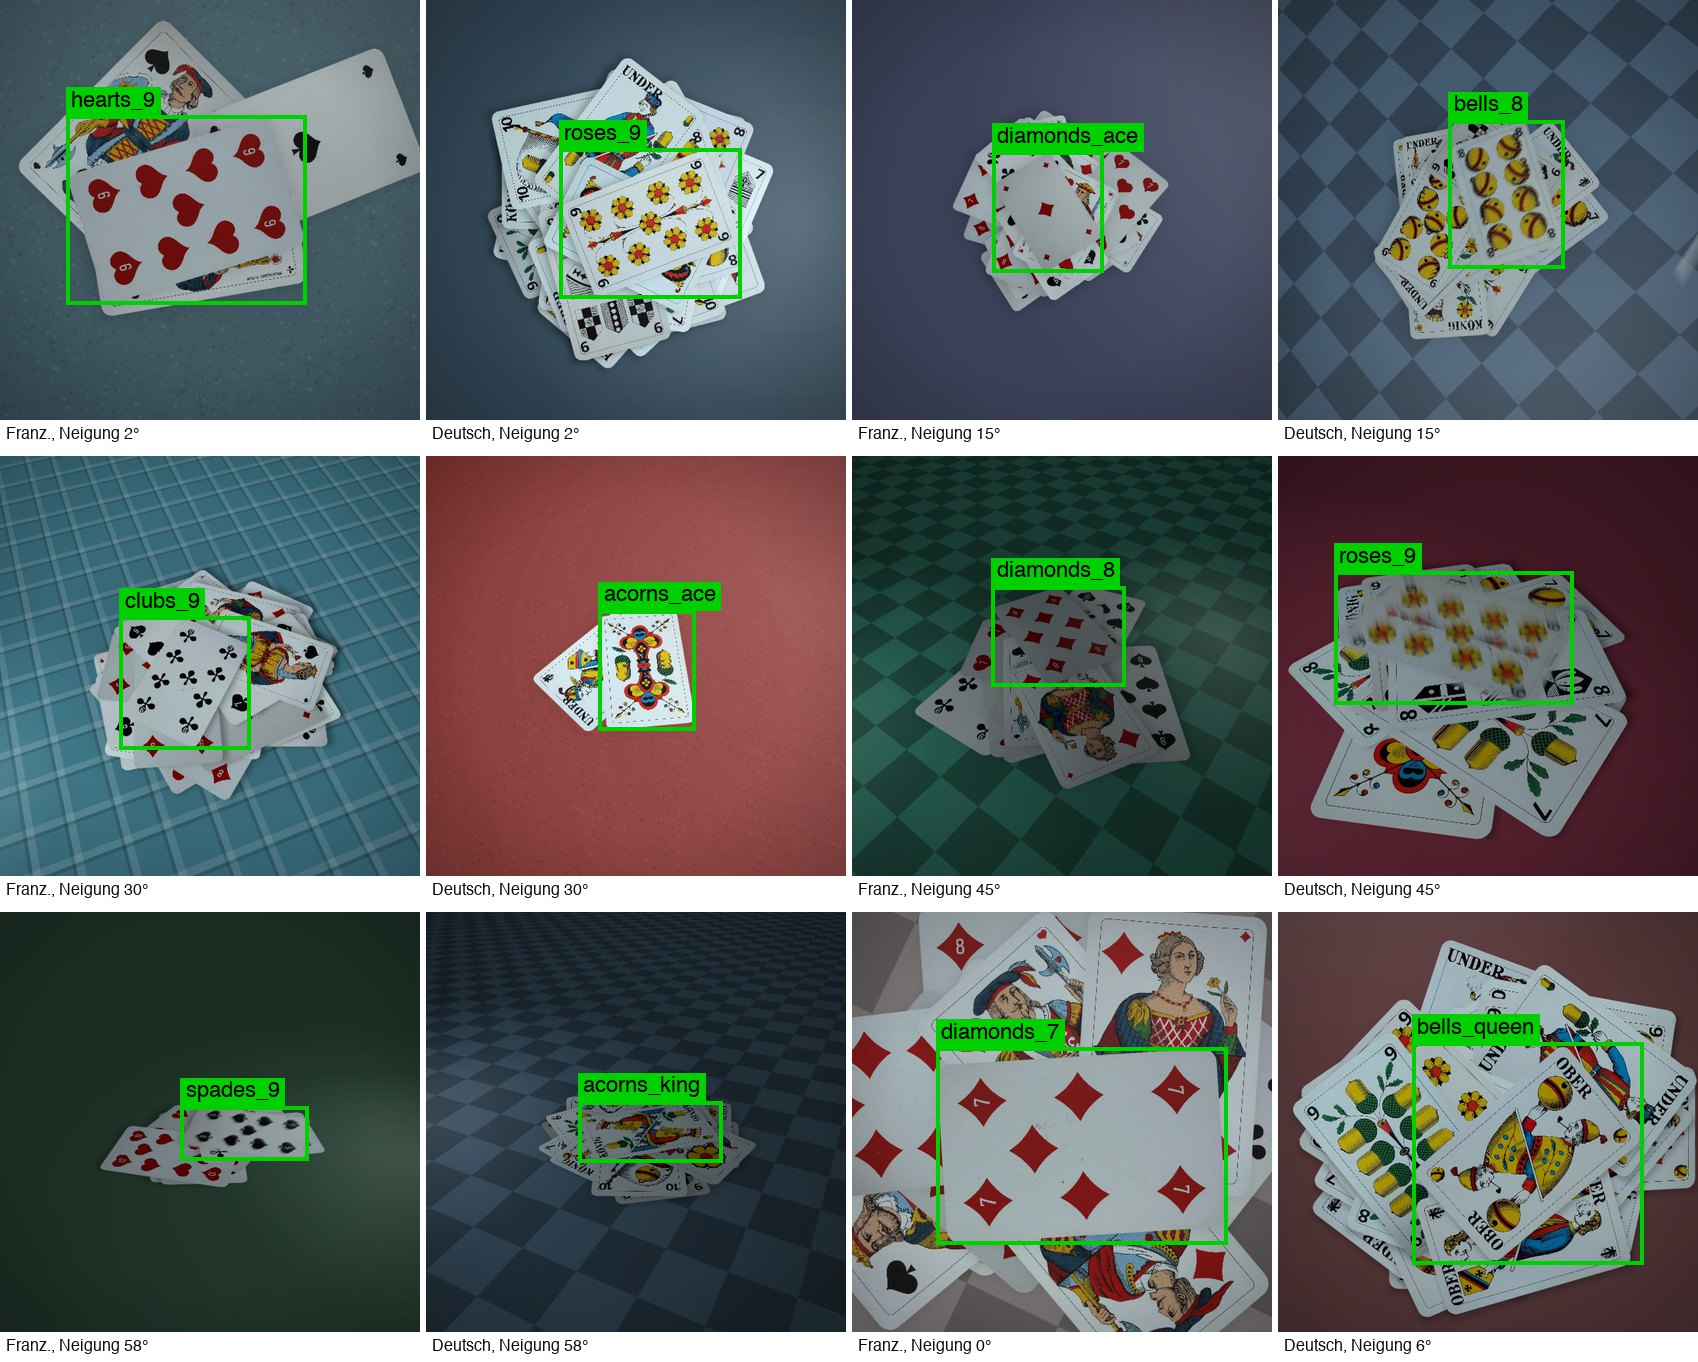
\includegraphics[width=0.85\textwidth]{synthetisch-beispiele.jpg}
\caption{Gerenderte Trainingsbilder beider Blätter mit der Box der obersten Karte (Variante~C). Der Winkel ist die Kameraneigung gegenüber der Senkrechten.}
\label{fig:synthetisch}
\end{figure}

\subsection{Kamerawinkel und Blatt aus dem Bildindex}\label{sec:sweep}

Bildindex $i$ und Bildanzahl $n$ legen die Kameraneigung und das
Kartenblatt fest. Die Neigung von Bild $i$ beträgt
\[
  \theta_i = 60^\circ \cdot \frac{p(i) + \tfrac{1}{2}}{n},
\]
wobei $p$ die Bildindizes permutiert. Die Bilder decken so den Bereich
von 0\textdegree{} bis 60\textdegree{} gleichmässig ab, ohne nach Winkel
sortiert zu sein. Bei grösseren Neigungen kann der Horizont ins Bild
geraten und die Tischprojektion fehlerhaft werden.

Gerade Positionen von $p(i)$ erhalten das französische Blatt, ungerade
das deutsche. Bei den verwendeten geraden Bildzahlen bekommt jedes Blatt
genau die Hälfte der Bilder und einen eigenen gleichmässigen Winkelsweep.
Ein Kartenhaufen enthält immer nur Karten desselben Blatts.

\subsection{Sichtbarkeitsregel}\label{sec:sichtbarkeit}

Eine Karte wird nur gelabelt, wenn sie vollständig im Bild liegt und
mindestens drei Pixel Abstand zum Rand hat. Sind höchstens 85\,\% ihres
projizierten Rechtecks sichtbar, gilt das Bild als Negativ. Szenen
dazwischen werden erneut gezogen. Bleibt der Fall nach 16 Versuchen
uneindeutig, entsteht ein Negativ. Die Wiederholung verringert
widersprüchliche Labels bei fast gleichen Bildern. Bei realen Fotos
werden klar
angeschnittene Karten als \enquote{No card} gespeichert. Berührt eine
fast vollständig sichtbare Karte nur den Rand, wird das Frame
ausgelassen.

\subsection{Negativbeispiele und Bewegungsunschärfe}\label{sec:negative}

Der Generator sieht für Negative einen Anteil von 30\,\% vor. Das liegt
bewusst über den 0 bis 10\,\% Hintergrundbildern, die Ultralytics
empfiehlt \cite{ultralytics2025tips}. Gerenderte
Negative zeigen einen leeren Tisch, eine stark verwischte geworfene Karte
oder eine verwischte Karte, die die oberste Karte verdeckt. Im Videostrom
der App kommen solche Frames häufig vor. Eine fälschlich gezählte Karte
wiegt dabei schwerer als eine übersehene. Die Detektoren erhalten für
Negative kein Label, der Klassifikator der Variante~A die Klasse
\code{none}.

Für Bewegungsunschärfe wird die Karte entlang ihrer Bewegungsrichtung
mehrfach gezeichnet. Bei 30\,\% der positiven Bilder beträgt die
Bewegungsstrecke 0.02 bis 0.09 Kartenhöhen. Diese Karten bleiben lesbar.
Stark verwischte Karten mit 0.25 bis 0.65 Kartenhöhen gehören zu den
Negativen. Der Bereich dazwischen wird nicht erzeugt. Ein Viertel der
positiven Bilder zeigt zudem eine verwischte Karte am Bildrand, während
die oberste Karte klar sichtbar bleibt. In 5\,\% der Szenen liegt statt eines
gestreuten Haufens ein bündig gestapeltes Deck.

Rund ein Viertel der Negative stammt aus 25 realen Fotos ohne Karte.
Sie zeigen unter anderem Papier, Kassenbons, Schachteln, Tische und
Räume. Zufällige Ausschnitte, Drehungen, Spiegelungen und wechselnde
Belichtung machen daraus viele Trainingsbilder. Diese Fotos ergänzen
die gerenderten Negative um Alltagsgegenstände, die sonst als Karte
fehlgedeutet werden könnten.

\subsection{Label-Varianten und Datensatz-Layout}\label{sec:layout}

Aus einem Renderlauf schreibt der Generator alle Label-Formate der drei
Varianten (Tabelle~\ref{tab:labelvarianten}). Die Bilder werden einmal
gerendert und von den Varianten gemeinsam genutzt.

\begin{table}[H]
\centering\small
\begin{tabularx}{\textwidth}{@{}llYl@{}}
\toprule
\textbf{Variante} & \textbf{Ordner} & \textbf{Label} & \textbf{Klassen} \\
\midrule
C & \code{detect/} & achsenparallele Box \code{klasse cx cy w h}, eine je Bild & 72 \\
B$_1$ & \code{locate/} & orientierte Box aus vier Eckpunkten & 1 \\
B$_2$ & \code{classify\_crop/} & entzerrter Kartenausschnitt in einem Klassenordner & 72 \\
A & \code{classify\_full/} & ganzes Bild in einem Klassenordner, Negative unter \code{none} & 73 \\
\bottomrule
\end{tabularx}
\caption{Die vier Label-Varianten aus einem Renderlauf.}
\label{tab:labelvarianten}
\end{table}

Für Variante~B$_2$ wird die oberste Karte anhand ihrer vier Ecken per
Homographie zu einem aufrechten Bild von 384 Pixeln Höhe entzerrt. Im
Betrieb geschieht dies anhand der Vorhersage der ersten Stufe. Innerhalb
eines Datensatzes bilden Bilder, Detektions- und Lokalisierungslabels
sowie die Klassenliste die Grundlage. Abgeleitete Klassenordner und
die \code{data.yaml} werden bei Bedarf mit \code{rebuild} rekonstruiert.

\subsection{Qualitätssicherung der Labels}\label{sec:label-qa}

Automatische Konsistenzprüfungen und die Sichtung aller entzerrten
Ausschnitte fanden drei falsche Klassenlabels unter 211 geprüften Bildern.
Sie wurden korrigiert. Bei einigen Kreuz- und Schaufelkarten begann die
Vier-Ecken-Annotation an der falschen Ecke. Das dreht nur den entzerrten
Ausschnitt für B$_2$ um 180\textdegree{}. Die Boxen von C und B$_1$ bleiben
gleich. Automatische Korrekturversuche erzeugten zu viele Fehlmarkierungen,
daher wurden die Ausschnitte visuell geprüft. Dabei fielen auch zwölf
verdrehte französische Kartenscans auf, die korrigiert wurden.

\section{Training und mobile Umsetzung}\label{sec:training}

\subsection{Trainingsrezept}\label{sec:rezept}

Ein Python-Skript trainiert die vier Modelle der drei Ansätze mit
Ultralytics 8.3.155 \cite{jocher2024ultralytics}. Es läuft auf
NVIDIA-GPUs mit CUDA, auf dem Mac mit Apple MPS oder auf der CPU.
Als Ausgangspunkt dienen
vortrainierte Gewichte von YOLO11n für die Detektion, YOLO11n-obb für
orientierte Boxen und YOLO11n-cls für die Klassifikation.

Ein Lauf umfasst normalerweise 20 Epochen mit einer Bildgrösse von
640 Pixeln. Auf dem Mac werden 16 Bilder pro Batch verarbeitet, auf der
Cloud-GPU 64. Ultralytics erhöht die Lernrate während der ersten drei
Epochen schrittweise. Bei den Detektoren wird die Mosaic-Augmentierung
in den letzten zehn Epochen abgeschaltet. Die Voreinstellung für einen
vorzeitigen Abbruch liegt bei 100 Epochen und greift bei diesen Läufen
nicht \cite{ultralytics2026cfg}.

Horizontale und vertikale Spiegelungen sind deaktiviert, weil eine
gespiegelte Karte eine andere Karte ergibt. Die Klassennamen stammen
aus der gemeinsamen Kartenliste. Bei den Klassifikatoren ordnet
Ultralytics die Klassen intern alphabetisch. Deshalb lesen die Apps
die zum Modell gehörenden Klassennamen, statt sich auf die
Klassenindizes zu verlassen.

Trainiert wird auf synthetischen Bildern. Nach jeder Epoche wird auf
realen Fotos validiert. Die Gewichte der besten Epoche werden als
\code{best.pt} gespeichert. Weil diese Epoche anhand desselben
Validierungssets gewählt wird, auf dem die Ergebnisse berichtet
werden, können die Kennzahlen etwas zu hoch ausfallen
(Abschnitt~\ref{sec:grenzen}).

\subsection{Reproduzierbare Trainingspipeline}\label{sec:pipeline}

Die ersten Modelle wurden auf einem MacBook trainiert. Für grössere
Datensätze und den Vergleich aller Varianten kamen gemietete
Cloud-GPUs zum Einsatz. Ein GitHub-Actions-Workflow startet dafür
einen RunPod-Pod. Dieser lädt den festgelegten Commit, erzeugt den
Datensatz aus Seed und Bildanzahl und trainiert die Varianten
nacheinander. Während des Laufs werden Manifest, Log, Gewichte und
Metriken in Azure Blob Storage gespeichert. Ein lokales Werkzeug
holt die Ergebnisse zurück und exportiert das gewählte Modell für
beide Apps.

Die Trainingsbilder werden für jeden Lauf neu erzeugt. Grundlage sind
der versionierte Code, die Kartenscans und die festgelegten
Generatorparameter (Abschnitt~\ref{sec:repro}). Das Manifest hält
Commit, Seed, Bildanzahl und Konfiguration fest. Ein Wächter prüft
halbstündlich, ob die Läufe noch Fortschritte melden, und beendet
verwaiste Pods. Die Pipeline ist in
\code{src/training/pipeline.md} dokumentiert.

\subsection{Export und mobile Inferenz}\label{sec:app}

Aus \code{best.pt} entstehen zwei Modelle mit denselben trainierten
Gewichten. Für die eingereichten Apps wird Variante~C verwendet.
Ihr Core-ML-Modell enthält die Non-Maximum Suppression, sodass Vision
fertige Boxen liefert. Ultralytics speichert dieses Modell in halber Genauigkeit
(FP16) \cite{ultralytics2026coreml}. Für Android entsteht ein LiteRT-Modell in voller Genauigkeit
(FP32) ohne diesen Schritt. Die App wertet dessen Ausgabe selbst
aus. Bei der Berechnung auf einer Android-GPU kann LiteRT
trotzdem mit FP16 rechnen \cite{google2026litertgpu}.

Eine zusätzliche Quantisierung auf 8 Bit wurde nicht vorgenommen.
Das Core-ML-Modell ist 5.3\,MB gross. Das LiteRT-Modell benötigt aufgrund
der vollen Genauigkeit 10.7\,MB. Um die Geschwindigkeit in der App
einzuschätzen, wurde die Laufzeit pro Bild auf vier verfügbaren
Smartphones gemessen (Tabelle~\ref{tab:geraete}). Auf den beiden iPhones
dauert die Erkennung 15 beziehungsweise 30\,ms. Das Pixel~7a erreicht mit
50\,ms genau den festgelegten Zielwert. Auf dem Nexus~5X benötigt die
Verarbeitung dagegen rund drei Sekunden pro Bild. Damit lässt sich die
App auf diesem Gerät nicht sinnvoll bedienen.

Die Werte sind gerundete Einzelmessungen und dienen nur als grobe
Einordnung. Sie erlauben keinen allgemeinen Vergleich zwischen iOS und
Android. Arbeitsspeicher und Energieverbrauch wurden nicht gemessen. Für
schwächere Android-Geräte bleibt eine Quantisierung auf 8 Bit eine
mögliche Erweiterung (Abschnitt~\ref{sec:ausblick}).

\begin{table}[H]
\centering\small
\begin{tabular}{@{}lclr@{}}
\toprule
\textbf{Gerät} & \textbf{Jahr} & \textbf{Laufzeitumgebung} & \textbf{Zeit pro Bild} \\
\midrule
iPhone 17 Pro Max & 2025 & Core ML & 15\,ms \\
iPhone 14 Pro & 2022 & Core ML & 30\,ms \\
Google Pixel 7a & 2022 & LiteRT & 50\,ms \\
Nexus 5X & 2015 & LiteRT & 3000\,ms \\
\bottomrule
\end{tabular}
\caption{Gerundete Laufzeit der Variante~C pro Bild. Die Werte stammen aus
einer Einzelmessung in der jeweiligen App.}
\label{tab:geraete}
\end{table}

Die Klassennamen sind Teil des Exports. Die Datei \code{models.json}
nennt für jedes gebündelte Modell den Trainingslauf und den Commit.

Die App wurde mit SwiftUI für iOS und mit Kotlin und Jetpack Compose
für Android umgesetzt. Beide verwenden im Kamerabild das grösste
mittige Quadrat und skalieren es auf 640 Pixel. Damit entspricht
der Bildausschnitt dem Format der Trainingsbilder. Für den
Variantenvergleich konnte die iOS-Implementierung auch A und B
verarbeiten. Bei B entzerrt sie den von der ersten Stufe gefundenen
Ausschnitt und klassifiziert ihn danach. Die eingereichten Apps
enthalten Variante~C.

\subsection{Von der Erkennung zur gezählten Karte}\label{sec:zaehlung}

Aus dem geplanten Proof of Concept ist eine fertig implementierte
Zähl-App für iOS und Android geworden. Beide Versionen wurden am
14.\,September als Version 1.0.0 im App Store und bei Google Play
eingereicht. Sie sind als Gratis-Demo mit einmaligem Kauf angelegt.
Die Kaufabwicklung, Store-Texte und Screenshots gingen über den
geplanten Proof of Concept und den Untersuchungsrahmen dieser Arbeit
hinaus. Ziel ist, die App interessierten Personen am Tag der
Präsentation zugänglich zu machen. Die guten Erkennungsresultate
sprechen dafür, die App danach weiterzuentwickeln und zu pflegen.

Eine Erkennung wird noch nicht sofort gezählt. Die App verwirft
Vorhersagen mit einer Konfidenz unter 0.6. Danach prüft sie, ob
dieselbe Karte in mehreren Frames erscheint. Standardmässig muss
sie in drei aufeinanderfolgenden Frames die beste Erkennung sein
(\enquote{Serie}). Als Alternative reichen drei von fünf Frames,
solange keine andere noch ungezählte Karte mehr als einmal
erscheint (\enquote{Mehrheit}). Die benötigte Anzahl lässt sich
von 1 bis 10 einstellen. Schwelle und Standardeinstellung der
Stabilitätsregel wurden zunächst ohne Messung gewählt. Ihre
Wirkung wurde später an einer aufgezeichneten Session geprüft
(Abschnitt~\ref{sec:betriebspunkt}).

Vor der Zählung werden das Kartenblatt und die Spielart gewählt. Danach
öffnet sich die Kamera. Die App
berücksichtigt nur die 36 Karten dieses Blatts und verhindert
Doppelzählungen. Der Stapel lässt sich durch Antippen korrigieren.
Die Punkte werden nach neun Spielarten aus drei Wertetabellen
berechnet. Ein Prüfskript kontrolliert diese Tabellen in der
Continuous Integration.
Für jede gezählte Karte gibt die App ein Signal. Ein verborgener
Entwicklermodus kann die Zählung als Video und als
Erkennungsprotokoll je Frame aufzeichnen. Diese Aufnahmen dienen
der Auswertung in Abschnitt~\ref{sec:betriebspunkt}.

\section{Ergebnisse und Auswertung}\label{sec:experimente}

Dieses Kapitel beantwortet die zwei Forschungsfragen anhand der letzten
Datenmengenreihe. Die Modelle wurden ausschliesslich auf synthetischen
Bildern trainiert und auf dem aktuellen realen Validierungsset geprüft.
Zum Schluss wird die Erkennung in der App eingeordnet.

\subsection{Die gemeinsame Datenmengenreihe}\label{sec:saettigung}

Für die Reihe wurden sechs Datensätze mit 5'000, 10'000, 20'000, 50'000,
100'000 und 200'000 Bildern erzeugt. Bei jeder Bildanzahl wurden alle vier
Modelle der Ansätze A, B und C trainiert. Generatorstand, Seed,
Modellgrösse, Bildauflösung und Trainingsplan blieben gleich. Alle Modelle
wurden auf denselben 813 realen Frames ausgewertet. Davon zeigen 513
eine gelabelte Karte und 300 gelten als Negative.

Um zu prüfen, ob noch mehr Bilder weiterhelfen, wurde Variante~C
zusätzlich mit 500'000 Bildern trainiert. Generator, Seed,
Trainingsplan und Validierungsset sind dieselben. Der Lauf stammt von
einem späteren Commit, der nur den Speicherplatz der Trainingsmaschine
vergrösserte. Für A und B liegt bei dieser Bildanzahl kein Wert vor.

Die Datensätze sind keine ineinander enthaltenen Teilmengen. Die
Bildanzahl beeinflusst auch den Winkelplan und die Verteilung der
Kartenblätter (Abschnitt~\ref{sec:repro}). Innerhalb der Reihe lässt sich
dennoch untersuchen, wie sich die Leistung bei grösseren Datensätzen
entwickelt. Abbildung~\ref{fig:saettigung} zeigt die Ergebnisse.

\begin{figure}[H]
\centering
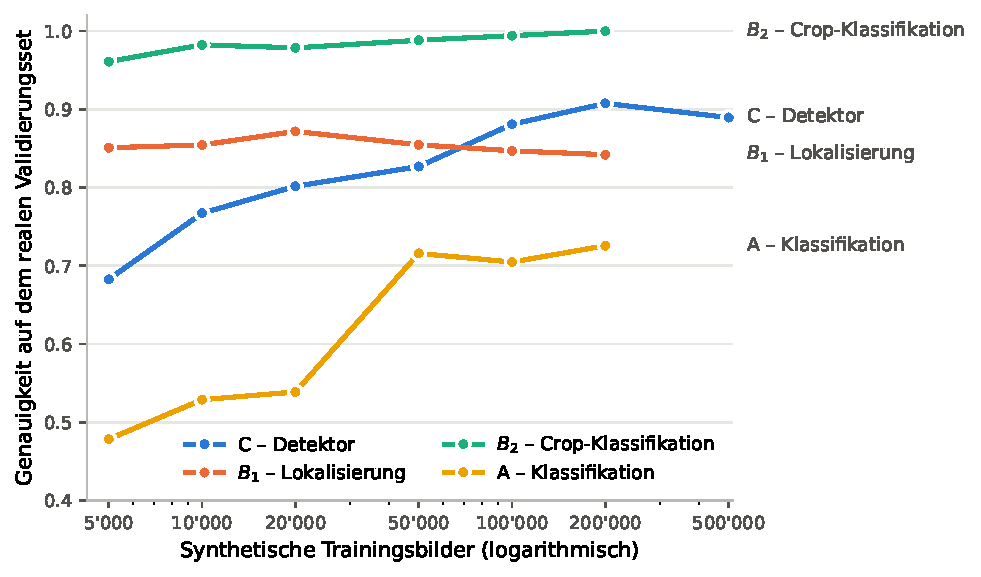
\includegraphics[width=0.92\textwidth]{saettigung.pdf}
\caption{Ergebnisse der sechs Datenmengen auf demselben realen
Validierungsset, für C zusätzlich mit 500'000 Bildern. Für C und B$_1$ wird \map{50} gezeigt, für A und B$_2$
die Top-1-Genauigkeit. Die Höhen dieser verschiedenen Kennzahlen sind
nicht direkt vergleichbar. B$_2$ erhält ideal entzerrte Ausschnitte.}
\label{fig:saettigung}
\end{figure}

Abbildung~\ref{fig:verlauf} zeigt den Trainingsverlauf von Variante~C.
Mit 5'000 Bildern verbessert sich das Modell während fast des gesamten
Trainings und erreicht erst gegen Ende sein bestes Ergebnis von 0.683.
Bei grösseren Datensätzen steigt der Wert schneller an. Ab 50'000
Bildern liegt die \map{50} bereits nach wenigen Epochen über 0.7 und
verändert sich danach nur noch wenig.

Bei den drei grössten Datensätzen wird das beste Ergebnis zwischen
Epoche 10 und 13 erreicht. Danach nimmt die Leistung wieder leicht ab.
Beim Lauf mit 200'000 Bildern endet sie bei 0.826 statt beim Höchstwert
von 0.908. Exportiert wird deshalb \code{best.pt} mit den Gewichten der
besten Epoche.

\begin{figure}[H]
\centering
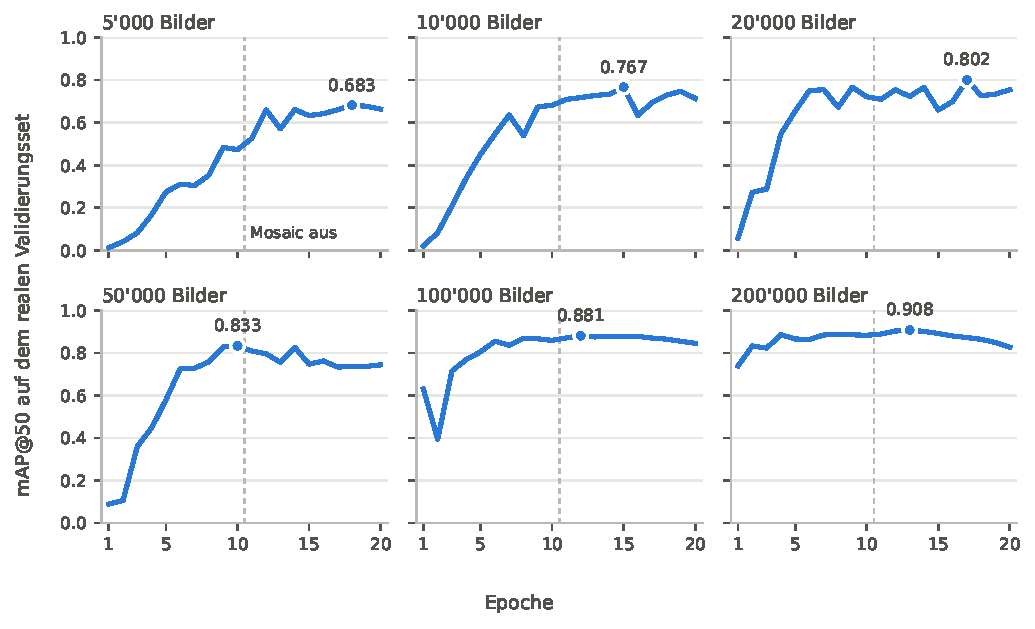
\includegraphics[width=0.92\textwidth]{trainingsverlauf.pdf}
\caption{\map{50} der Variante~C auf dem realen Validierungsset je Epoche,
ein Feld je Datensatzgrösse. Der Punkt markiert die beste Epoche. Ab der
gestrichelten Linie ist die Mosaic-Augmentierung abgeschaltet.}
\label{fig:verlauf}
\end{figure}

\subsection{Vergleich der Erkennungsansätze (FF1)}\label{sec:vergleich}

Der einstufige Detektor C wird mit mehr Trainingsbildern bis 200'000
Bilder stetig besser und erreicht dort auf den realen Frames eine
\map{50} von 0.908. Bis hierhin passt der Verlauf zur Beobachtung von
Sun et al., dass die Leistung von Bildmodellen mit dem Logarithmus der
Datenmenge steigt \cite{sun2017revisiting}. Mit 500'000 Bildern liegt
die \map{50} bei 0.889. Mehr Bilder aus demselben Generator bringen
also keinen weiteren Gewinn. Der Abstand von 0.019 ist bei einem
einzelnen Seed nicht als Rückgang zu deuten
(Abschnitt~\ref{sec:setup}). Der Detektor gibt die Kartenklasse und ihre Position mit einem
Modell aus. Die reine Klassifikation A verbessert sich ebenfalls, liefert
aber keine Position der Karte.

Beim zweistufigen Ansatz B erkennt B$_1$ zuerst die Position der Karte.
Seine \map{50} verändert sich mit mehr Bildern nur wenig und liegt am Ende
der Reihe bei 0.842. B$_2$ klassifiziert einen ideal entzerrten
Kartenausschnitt fast immer richtig. Diese Ausschnitte stammen aus den von
Hand gesetzten Ecken. Im Betrieb muss B$_2$ dagegen mit den Vorhersagen von
B$_1$ arbeiten. Fehler beim Finden oder Entzerren der Karte wirken sich
dann auf die Klassifikation aus. Die letzte Reihe enthält keine
verlässliche Messung dieser gesamten Verarbeitungskette. Für B lässt
sich deshalb keine Trefferquote für die vollständige Erkennung angeben.

Für die mobile Nutzung spricht die vorliegende Evidenz am stärksten für C.
Ein weiterer Vorteil zeigt sich direkt bei der Bedienung. Die
achsenparallele Box umschliesst eine schräg liegende Karte zwar nicht
genau. Sie zeigt beim Zählen dennoch, welche Karte erkannt wurde und wo
sie sich im Bild befindet. Diese Rückmeldung fehlt bei A. Dadurch wirkt
eine Erkennung teilweise ungewohnt, weil ihr Bezug zum Kamerabild nicht
sichtbar ist. B benötigt zwei Modelle und einen zusätzlichen
Entzerrungsschritt. C übernimmt die Erkennung der Kartenklasse und ihrer
Position mit einem Modell und läuft in den eingereichten Apps auf
aktuellen Geräten in Echtzeit (Tabelle~\ref{tab:geraete}).
Ein neuer, gemeinsamer Latenzvergleich aller Varianten auf demselben Gerät
liegt für diese Reihe nicht vor. Der genaue Abstand beim Rechenaufwand
bleibt damit offen.

\subsection{Übertragung auf reale Aufnahmen (FF2)}\label{sec:transfer-real}

Das beste Ergebnis von C in der Datenmengenreihe stammt von einem Modell,
das keine realen Kartenhaufen als Trainingsbilder gesehen hat. Seine
\map{50} von 0.908 auf den realen Aufnahmen zeigt, dass die synthetischen
Bilder für die Erkennung auf diesem Validierungsset geeignet sind. Die
Kennzahl berücksichtigt die richtige Kartenklasse und die Überlappung
der erkannten Position mit dem Label. Sie ist nicht gleichbedeutend mit
dem Anteil richtig gezählter Karten in einer Zählsession.

Im Projektverlauf wurden Generator und reale Prüfbasis erweitert.
Insbesondere flache Kamerawinkel erhielten mehr Gewicht. Der Generator
deckt nun Neigungen bis 60\textdegree{} ab. Hinzu kamen Aufnahmen unter
anderen Lichtverhältnissen, beide Kartenblätter und schwierigere
Negativbeispiele. Die reale Prüfbasis enthält ebenfalls mehr flache
Perspektiven und Situationen ohne klar lesbare Karte. Diese Änderungen
verbessern die Abdeckung der vorgesehenen Einsatzbedingungen. Ihr
einzelner Beitrag zur Modellleistung wurde nicht getrennt gemessen.

Die Aussage zum Transfer gilt zunächst nur für die vorhandenen
Aufnahmen. Viele Frames stammen aus denselben Videos und ähneln sich.
Ausserdem wurde die beste Trainingsepoche anhand dieses
Validierungssets gewählt. Ein unabhängiges Testset und Wiederholungen
mit weiteren Trainings-Seeds fehlen. Besonders bei Karten im Wurf oder
an der Grenze zwischen lesbar und unlesbar bleibt auch die Bewertung
schwierig (Abschnitt~\ref{sec:grenzfaelle}).

\subsection{Betrieb in der App}\label{sec:betriebspunkt}

Die eingereichten Apps verwenden Variante~C. Eine Karte wird erst
gezählt, wenn die Erkennung die eingestellte Konfidenz erreicht und über
mehrere Frames stabil bleibt (Abschnitt~\ref{sec:zaehlung}). Eine
aufgezeichnete Zählsession wurde im Dataset Tool mit verschiedenen
Einstellungen erneut ausgewertet. Dabei zeigte sich, dass einzelne
Fehler auch mit einer hohen Konfidenz auftreten können
(Abbildung~\ref{fig:frames-nacheinander}). Eine höhere Schwelle allein
löst dieses Problem daher nicht. Die Stabilitätsregel hilft, solche
kurzen Ausreisser abzufangen.

\begin{figure}[H]
\centering
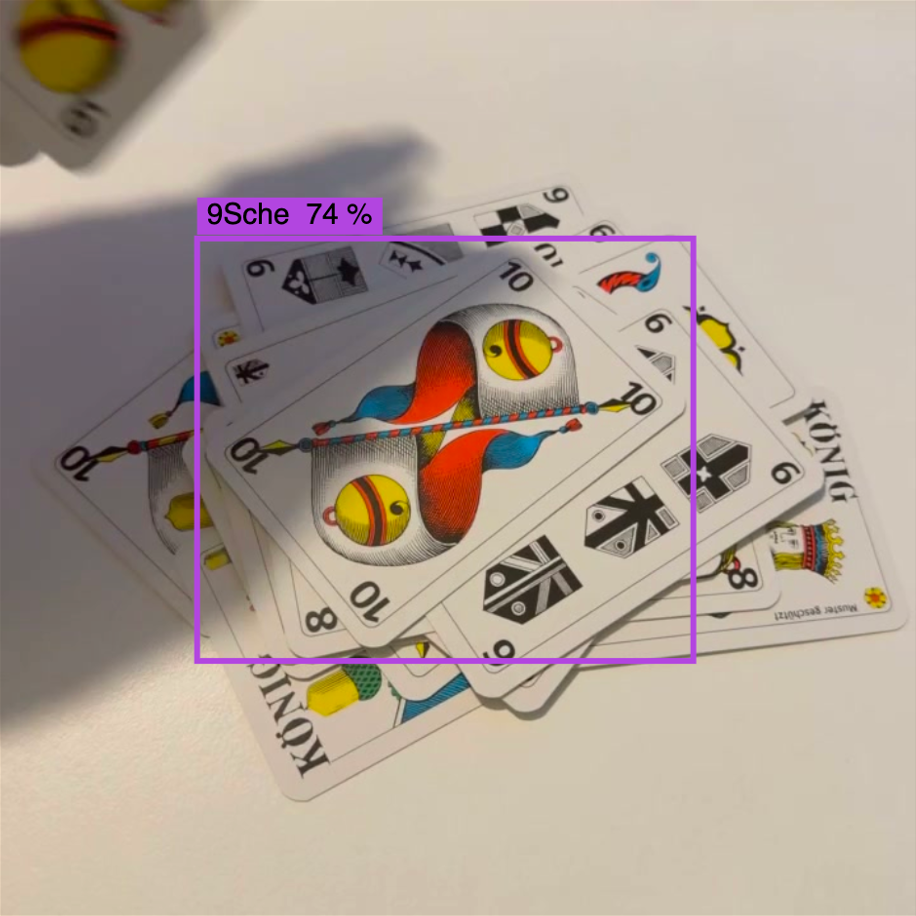
\includegraphics[width=0.48\textwidth]{detection-difficulties-wrong.png}\hfill
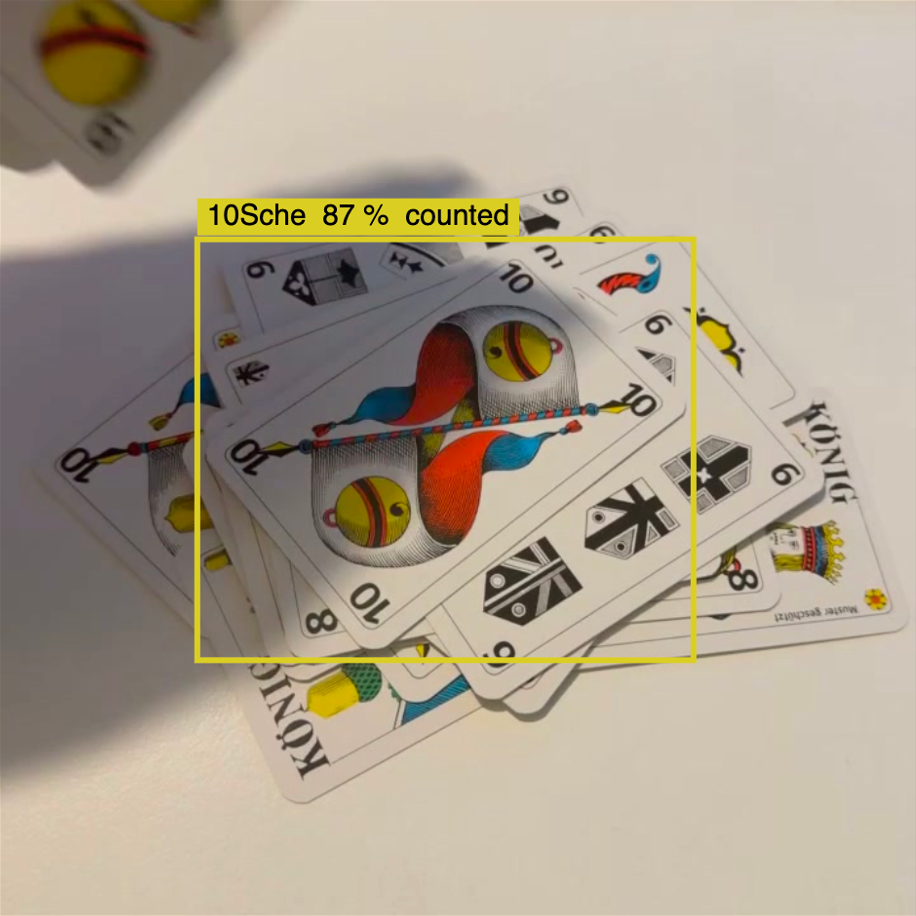
\includegraphics[width=0.48\textwidth]{detection-difficulties-correct.png}
\caption{Zwei direkt aufeinanderfolgende Frames derselben Aufnahme. Links
erkennt das Modell die oberste Karte mit 74\,\% fälschlich als Schellen~9.
Diese Erkennung wird nicht gezählt. Im nächsten Frame erkennt es die
Schellen~10 mit 87\,\% korrekt und die App zählt die Karte. Die gelbe
Markierung zeigt die gezählte Erkennung. Der Kartenhaufen und die Position der
Kamera haben sich zwischen den beiden Frames kaum verändert.}
\label{fig:frames-nacheinander}
\end{figure}

Diese einzelne Session reicht nicht für eine verlässliche Erfolgsquote.
Sie zeigt jedoch, wie sich die Einstellungen der App anhand einer
vollständigen Aufnahme prüfen lassen. Für aussagekräftige Ergebnisse
braucht es weitere Sessions mit unterschiedlichen Geräten und
Spielsituationen. Dabei sollten ganze Zählvorgänge statt nur einzelne
Frames ausgewertet werden.

\section{Diskussion und Reflexion}\label{sec:diskussion}

\subsection{Beantwortung der Forschungsfragen}\label{sec:antworten}

\paragraph{FF1, Erkennungsansatz.} Variante~C ist für die App die am besten
belegte Wahl. In der letzten Datenmengenreihe erreicht der Detektor bei
200'000 Trainingsbildern auf dem realen Validierungsset eine \map{50} von
0.908. Er liefert Kartenklasse und Position mit einem Modell und läuft in
den eingereichten Apps in Echtzeit. Variante~A liefert keine Position.
Bei Variante~B sind die Lokalisierung und die Klassifikation ideal
entzerrter Ausschnitte gemessen, aber nicht die gesamte Erkennungskette.
Zudem fehlt für die letzte Reihe ein Latenzvergleich aller Ansätze auf
demselben Gerät. Wie gross der Vorteil von C bei Genauigkeit und
Rechenaufwand tatsächlich ist, lässt sich daher nicht beziffern.

\paragraph{FF2, Übertragung auf reale Aufnahmen.} Das Modell C wurde nur
mit synthetischen Bildern trainiert und erkennt Karten auf den eigenen
realen Aufnahmen. Damit funktioniert die Übertragung für das vorhandene
Validierungsset. Im Projekt wurden die Trainingsbilder und die reale
Prüfbasis schrittweise um flachere Perspektiven, andere
Lichtverhältnisse und schwierigere Negativbeispiele erweitert. Diese
Änderungen wurden nicht einzeln unter gleichen Bedingungen gemessen.
Wie gut das Modell auf neuen Aufnahmesessions oder anderen
Kartendesigns arbeitet, bleibt offen.

\subsection{Grenzen der Ergebnisse}\label{sec:grenzen}

Das Validierungsset enthält 813 Frames, davon 513 mit gelabelter Karte.
Viele Frames stammen aus denselben Videos und ähneln sich. Ausserdem
wird die beste Trainingsepoche auf diesem Set ausgewählt und dort auch
bewertet. Ein unabhängiges Testset und Wiederholungen mit weiteren
Trainings-Seeds fehlen. Die Kennzahlen können deshalb zu günstig
ausfallen. Kleine Unterschiede zwischen den Modellen sind nicht als
gesicherte Effekte zu verstehen.

Die Datenmengenreihe verwendet für jede Bildzahl denselben Generator
und Trainingsplan. Die Datensätze sind aber keine ineinander
enthaltenen Teilmengen. Mit der Bildzahl ändert sich auch, welche
Winkel und Kartenblätter auf die einzelnen Bilder fallen. Der
beobachtete Verlauf zeigt, was die grösseren Datensätze dieser Reihe
leisten. Er trennt den Einfluss der reinen Bildanzahl nicht vollständig
vom Einfluss der gezogenen Bilder.

Die Modelle werden mit unterschiedlichen Kennzahlen beurteilt.
\map{50} für die Detektoren und Top-1-Genauigkeit für die
Klassifikatoren dürfen nicht als dieselbe Trefferquote gelesen
werden. Vor allem sagt keine dieser Kennzahlen direkt, wie oft die
App einen ganzen Stapel richtig zählt.

Auch die Trainingsbilder haben Grenzen. Die Kartenscans stammen aus je
einem physischen Deck pro Blatt. Der Generator verändert Perspektive,
Licht und Hintergrund, aber nicht das Kartendesign. Hände, gekippte
Karten, harte Schatten und Spiegelungen auf glänzenden Karten fehlen.
Für solche Situationen und andere Decks braucht es zusätzliche reale
Prüfaufnahmen.

\subsection{Kurskorrekturen im Projekt}\label{sec:verworfen}

Zuerst sollten die Trainingsbilder fotografiert und von Hand gelabelt
werden. Für die benötigte Menge war das nicht praktikabel. Der Wechsel
zu gerenderten Bildern machte grössere Datensätze und automatische
Labels möglich. Reale Fotos dienen nun als Quellmaterial und zur
Prüfung, nicht als Trainingsbilder für Kartenhaufen.

Generator und Validierungsset wurden während des Projekts erweitert.
Besonders Aufnahmen aus flacheren Winkeln und Bilder ohne eindeutig
lesbare Karte zeigten, welche Situationen noch fehlten. Daraufhin
wurden die Kamerawinkel und die Negativbeispiele breiter angelegt.
Diese Schritte gehören zur Entwicklung des Systems. Da sie nicht
einzeln geprüft wurden, lässt sich ihnen keine bestimmte
Leistungssteigerung zuordnen. Entscheidend ist, dass die reale
Prüfbasis nicht nur Fälle zeigt, die der Generator bereits gut
abbildet.

Auch die Einstellungen der App mussten genauer betrachtet werden.
Konfidenzschwelle und Stabilitätsregel waren zunächst gesetzt, ohne
dass ihre Wirkung an mehreren Sessions gemessen worden war. Bei der
Prüfung zeigte sich zudem, dass die Apps die Konfidenz zeitweise
unterschiedlich auswerteten. Solche Werte müssen nachvollziehbar
festgehalten und mit aufgezeichneten Zählvorgängen geprüft werden.

\subsection{Eigene Werkzeuge}\label{sec:eigene-werkzeuge}

Das Dataset Tool verbindet die Sichtkontrolle der gerenderten Bilder,
das Labeln realer Aufnahmen und die Analyse von Zählsessions. Die
Dataset-CLI erzeugt und prüft die Daten. Beide Werkzeuge wurden für
die Fragen dieses Projekts gebaut. Dadurch liess sich eine Änderung
am Generator rasch an Bildern und Labels kontrollieren. Ein Label
kann zudem für alle drei Erkennungsansätze verwendet werden. Für
grössere Teams, die gemeinsam labeln und Ergebnisse gegenseitig
prüfen, wäre ein etablierter Dienst weiterhin sinnvoll.

\subsection{Rolle der KI und persönlicher Beitrag}\label{sec:ki-reflexion}

Der Code des Projekts wurde überwiegend mit Claude Code erstellt. Der
Verfasser legte die Aufgabe, die drei Ansätze, die Datenregeln und die
Architektur fest. Er fotografierte die Karten und die realen
Prüfaufnahmen, labelte die Daten, kontrollierte die erzeugten Bilder
und prüfte die Apps. Auch die Auswahl der Auswertungen und die
Interpretation der Ergebnisse lagen bei ihm. Die genaue Aufteilung
ist in Anhang~\ref{app:ki-deklaration} dokumentiert.

Die Arbeit mit KI machte die Umsetzung von Generator, Werkzeugen,
Trainingspipeline und zwei Apps in der verfügbaren Zeit möglich. Sie
nahm dem Verfasser die Prüfung nicht ab. Verdrehte Scans und Labels
fielen erst bei der Sichtkontrolle auf. Unterschiede bei der
Konfidenzauswertung der Apps mussten anhand der tatsächlichen
Ausgaben geprüft werden. Die Verantwortung für Annahmen, Messungen
und Schlussfolgerungen bleibt beim Verfasser.

\subsection{Lehren aus der Arbeit}\label{sec:lessons}

Eine reale Prüfbasis muss früh entstehen und mit neuen Fehlerfällen
wachsen. Die Regeln für lesbare, verdeckte und verwischte Karten
sollten vor dem Labeln feststehen. Ein reproduzierbarer Generator
hilft beim Vergleichen, ersetzt aber kein unabhängiges Testset.
Ebenso wichtig ist die Prüfung der vollständigen Zählung in der App.
Erst damit lässt sich beurteilen, ob gute Kennzahlen für einzelne
Frames auch zu einer verlässlichen Nutzung am Spieltisch führen.

\section{Schlussfolgerungen und Ausblick}\label{sec:schluss}

\subsection{Fazit}\label{sec:fazit}

Diese Arbeit zeigt, dass ein kleines Modell die oberste Karte eines
Jassstapels auf dem Smartphone in Echtzeit erkennen kann. Das Modell
wurde mit synthetischen Bildern aus den Scans zweier Kartenblätter
trainiert. In der letzten Datenmengenreihe erreicht der einstufige
Detektor C bei 200'000 Trainingsbildern auf dem realen
Validierungsset eine \map{50} von 0.908. Seine Leistung steigt bis
dorthin mit jeder Vergrösserung des Datensatzes. Ein zusätzlicher Lauf
mit 500'000 Bildern brachte keinen weiteren Gewinn. Die Menge der Bilder
aus diesem Generator ist damit ausgereizt.

Für die App ist C die am besten belegte Wahl. Es erkennt Klasse und
Position in einem Schritt. Die reine Klassifikation A liefert keine
Kartenposition. Für die vollständige zweistufige Erkennung B und
einen gemeinsamen Latenzvergleich liegen keine verlässlichen
Messungen aus der letzten Reihe vor. Deshalb lässt sich kein genauer
Leistungsabstand zwischen C und B angeben.

Der Transfer von synthetischen Trainingsbildern auf reale Aufnahmen
funktioniert auf dem vorhandenen Validierungsset. Wie zuverlässig
die App einen ganzen Stapel in neuen Spielsituationen zählt, ist
damit noch nicht gezeigt. Neben dem Modell sind ein Datengenerator,
eine reale Prüfbasis, eine Trainingspipeline und Zähl-Apps für iOS
und Android entstanden. Die Apps wurden in den Stores eingereicht.

\subsection{Ausblick}\label{sec:ausblick}

Als Nächstes soll das System mit neuen, unabhängigen Aufnahmesessions
geprüft werden. Dafür sollen ganze Zählvorgänge direkt in der App als
Video aufgezeichnet werden. Das Dataset Tool kann diese Sessions bereits
erneut abspielen und auswerten (Abbildung~\ref{fig:analyzer}). Künftig
soll diese Auswertung stärker automatisiert werden. Auffällige Frames
können direkt ins Validierungsset übernommen werden. Dadurch wird
sichtbar, welche Situationen in den Trainingsdaten noch fehlen und
gezielt ergänzt werden müssen.

\begin{figure}[H]
\centering
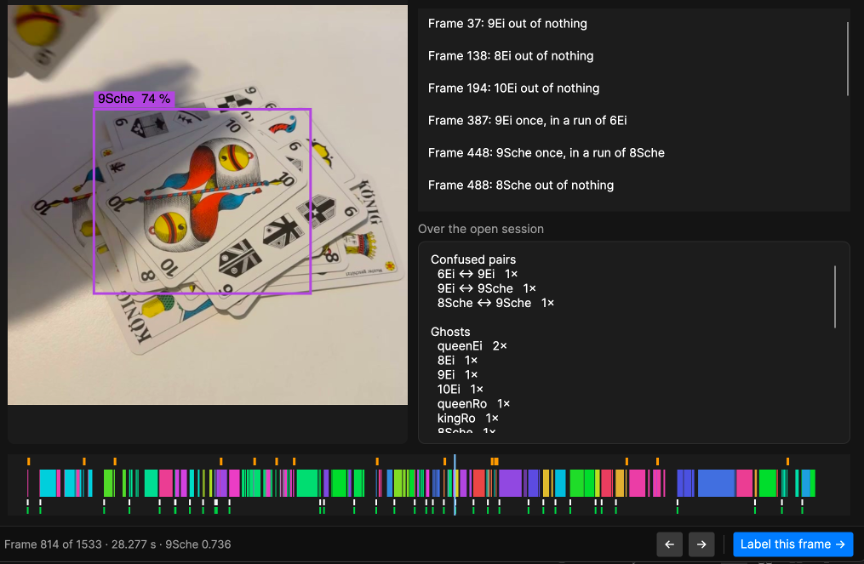
\includegraphics[width=\textwidth]{analyzer.png}
\caption{Auswertung einer aufgezeichneten Zählsession im Dataset Tool. Links
ist die Vorhersage für das ausgewählte Frame zu sehen. Rechts werden
auffällige Erkennungen und häufige Verwechslungen zusammengefasst. Über die
Zeitachse am unteren Rand lässt sich die gesamte Aufnahme prüfen. Das
ausgewählte Frame zeigt dieselbe falsche Erkennung wie das linke Bild in
Abbildung~\ref{fig:frames-nacheinander} und kann direkt ins Validierungsset
übernommen werden.}
\label{fig:analyzer}
\end{figure}

Auch die Labels des Validierungssets müssen möglicherweise genauer
unterteilt werden. Beim Labeln stellte sich immer wieder die Frage, ob
eine schwierige Karte noch erkannt werden muss oder bereits als
unlesbar gilt. Diese Entscheidung beeinflusst die Auswertung direkt.
Bei einigen Grenzfällen sind sowohl eine Erkennung als auch keine
Erkennung nachvollziehbar. Solche Aufnahmen könnten künftig gesondert
markiert und getrennt ausgewertet werden.

Für solche Grenzfälle gibt es ein etabliertes Vorbild. Die
PASCAL-VOC-Challenge markiert Objekte, die wegen ihrer Grösse, der
Beleuchtung, der Bildqualität oder des nötigen Kontextwissens besonders
schwer zu erkennen sind, mit einem eigenen Attribut. In der Auswertung
werden diese Objekte verworfen, und wer sie dennoch erkennt, wird dafür
nicht bestraft \cite{everingham2010pascal}.

YOLO kennt ein solches Attribut nicht. Das Labelformat sieht es nicht vor,
und Ultralytics verweist bei dieser Frage auf einen Eingriff in die
Verlustfunktion \cite{ultralytics2025ignore}. Die Markierung müsste
deshalb neben dem Validierungsset geführt und in einer eigenen Auswertung
berücksichtigt werden.

Aktuell werden beide Kartenblätter mit demselben Modell erkannt. Für
weitere Kartensets könnten stattdessen eigene Modelle pro Blatt
trainiert werden. Die App kennt das gewählte Kartenblatt bereits und
könnte das passende Modell laden. Dadurch liessen sich zusätzliche
Kartensets unabhängig voneinander ergänzen, ohne dass jedes Modell
immer mehr Klassen lernen muss.

Die Beschränkung auf die oberste Karte stellt zudem Anforderungen an
das Ablegen der Karten. Eine mögliche Erweiterung wäre, mehrere
vollständig sichtbare Karten gleichzeitig zu erkennen. YOLO kann
mehrere Objekte in einem Bild ausgeben. Die App müsste dabei
sicherstellen, dass jede Karte nur einmal gezählt wird.

Beim Testen zeigte sich ausserdem, dass das gleichzeitige Halten des
Smartphones und Ablegen der Karten umständlich sein kann. Zwei Personen
können diese Aufgabe aufteilen. Für eine einzelne Person wäre eine
einfache Halterung hilfreich. Sie könnte das Smartphone im richtigen
Winkel über dem Tisch halten und darunter eine Ablage für die gezählten
Karten bieten. Eine solche Vorrichtung würde die Bedienung vereinfachen
und für gleichmässigere Aufnahmen sorgen.


\clearpage
\section*{Glossar}
\addcontentsline{toc}{section}{Glossar}

\small
\begin{description}[style=unboxed, leftmargin=0pt, itemsep=1pt]
  \item[Augmentierung] Veränderung von Trainingsbildern. Bei der Mosaic-Augmentierung werden vier Bilder zusammengesetzt.

  \item[Bounding Box] Rechteck, das die Position eines Objekts im Bild beschreibt. Variante~C verwendet eine achsenparallele Box.

  \item[Core ML] Apples Laufzeit für Modelle auf iPhone und Mac.

  \item[Domain Randomization] Variation von Perspektive, Licht und Hintergrund beim Erzeugen synthetischer Trainingsbilder.

  \item[Epoche] Ein vollständiger Durchlauf des Modells durch die Trainingsbilder.

  \item[Fehlalarm] Vorhersage einer Karte in einem Frame, auf dem keine gültige oberste Karte erkannt werden soll. Eine falsch benannte vorhandene Karte ist ebenfalls ein Fehler, aber kein solcher Negativfall.

  \item[FP16 und FP32] Zahlenformate mit 16 beziehungsweise 32 Bit für Modellgewichte und Berechnungen.

  \item[Frame] Einzelbild eines Videos.

  \item[Homographie] Perspektivische Abbildung, die einen Kartenscan in die Szene verzerrt oder einen Kartenausschnitt aufrichtet.

  \item[Inferenz] Anwendung eines trainierten Modells auf ein neues Bild, um eine Vorhersage zu erhalten.

  \item[Intersection over Union (IoU)] Fläche, die sich vorhergesagte und gelabelte Box teilen, geteilt durch die Fläche, die beide Boxen zusammen bedecken. Der Wert liegt zwischen 0 und 1.

  \item[Konfidenzschwelle] Mindestwert, den eine Modellvorhersage erreichen muss, damit die App sie weiter berücksichtigt.

  \item[Label] Vorgegebene richtige Antwort zu einem Bild. Hier sind das die Kartenklasse und ihre Position oder die Markierung \enquote{No card}.

  \item[Latenz] Zeit, die das Modell und die zugehörige Verarbeitung für eine Vorhersage benötigen.

  \item[LiteRT] Googles Laufzeit für Modelle auf Android.

  \item[mAP] \emph{Mean Average Precision} ist der Mittelwert der Average Precision über die Kartenklassen. \map{50} verlangt eine IoU von 0.5. \map{50--95} mittelt über mehrere IoU-Schwellen.

  \item[Negativ] Bild oder Frame ohne gültige, lesbare oberste Karte. Auch eine stark verwischte Karte kann deshalb zu den Negativen gehören.

  \item[Non-Maximum Suppression (NMS)] Verarbeitungsschritt, der mehrere stark überlappende Vorhersagen für dasselbe Objekt auf eine Auswahl reduziert.

  \item[Orientierte Box (OBB)] Gedrehte Box, die hier durch die vier Ecken der Karte beschrieben wird. Variante~B nutzt sie für das Entzerren des Kartenausschnitts.

  \item[Precision und Recall] Precision ist der Anteil richtiger Meldungen an allen Meldungen des Modells. Recall ist der Anteil gefundener Karten an allen vorhandenen Karten.

  \item[Quantisierung] Darstellung von Modellwerten mit weniger Bits. Das kann die Ausführung beschleunigen, muss aber auf mögliche Änderungen der Erkennung geprüft werden.

  \item[Seed] Startwert für Zufallsentscheidungen bei Datenerzeugung oder Training. Ein festgelegter Seed macht die erzeugten Bildvarianten nachvollziehbar.

  \item[Session] Zusammenhängender Zählvorgang mit der App. Für die Auswertung kann er als Video mit Erkennungsprotokoll aufgezeichnet werden.

  \item[Sim-to-Real-Gap] Unterschied zwischen der Leistung auf synthetischen Bildern und auf realen Aufnahmen.

  \item[Stabilitätsregel] Regel der App, nach der dieselbe Karte erst über mehrere Frames hinweg erkannt werden muss, bevor sie gezählt wird.

  \item[Stich] Die Karten, die in einem Spielzug von einer Partei gewonnen werden. Die gewonnenen Stiche bilden den zu zählenden Stapel.

  \item[Testset] Aufnahmen für eine abschliessende Prüfung, die nicht zur Wahl des Modells oder seiner Einstellungen verwendet wurden.

  \item[Top-1-Genauigkeit] Anteil der Bilder, bei denen die Klasse mit dem höchsten Modellwert richtig ist.

  \item[Transfer Learning] Weiterverwendung vortrainierter Modellgewichte als Ausgangspunkt für eine neue Aufgabe.

  \item[Validierungsset] Bilder, mit denen während der Entwicklung Modelle verglichen und die beste Trainingsepoche ausgewählt werden. Es ist deshalb kein unabhängiges Testset.

  \item[YOLO] \emph{You Only Look Once}, eine Familie schneller Objektdetektoren. Hier wird YOLO11 verwendet.
\end{description}
\normalsize


\clearpage
\renewcommand{\refname}{Literaturverzeichnis}
\addcontentsline{toc}{section}{Literaturverzeichnis}
\bibliographystyle{alphadin}
\bibliography{literatur}

\clearpage
\appendix
\section{Deklaration des KI-Einsatzes}\label{app:ki-deklaration}

Im Rahmen dieser Arbeit wurden Claude Code von Anthropic und GPT-5.6 Sol
von OpenAI eingesetzt. Claude Code wurde als Agent für Agentic Coding
verwendet. Der Agent erhielt konkrete Arbeitsaufträge und konnte Dateien
im Repository erstellen oder ändern, Befehle ausführen und Tests starten.
Auf diese Weise entstand der grösste Teil der Dateien im Repository. Dazu
gehören der Datengenerator, das Dataset Tool, die Trainingspipeline, die
mobilen Apps sowie Skripte, Tests und Teile der projektbegleitenden
Dokumentation.

Die Arbeit mit Claude Code erfolgte in eng begleiteten Sitzungen. Der Verfasser
definierte jeweils die Anforderungen, Ziele und Randbedingungen. Danach
prüfte er die Änderungen im Code, führte Tests aus und kontrollierte die
erzeugten Ergebnisse. Jeder Commit wurde durch den Verfasser in einem
Review geprüft. Fehler, unklare Annahmen oder Abweichungen führten zu
einem neuen und genauer formulierten Arbeitsauftrag. Alle Entscheide zur
Architektur, zu den Daten, zum Training, zur Bedienung der Apps und zum
weiteren Vorgehen wurden durch den Verfasser getroffen.

Die vorliegende Transferarbeit wurde vom Verfasser selbst geschrieben.
Für die sprachliche Überarbeitung einzelner Textstellen wurde GPT-5.6 Sol
eingesetzt. Das Modell unterstützte bei der Korrektur von Grammatik und
Satzstellung, bei der stilistischen Verbesserung sowie bei der Prüfung
auf Richtigkeit. Alle vorgeschlagenen Änderungen wurden vom Verfasser
geprüft und bei Bedarf angepasst.

KI-Ausgaben werden in dieser Arbeit nirgends als Quelle zitiert. Aussagen,
die einen Beleg benötigen, verweisen auf die im Literaturverzeichnis
aufgeführten Quellen. Die Verantwortung für den Inhalt, die Entscheide,
die Ergebnisse und die Schlussfolgerungen liegt beim Verfasser.

\begin{table}[H]
\centering\small
\begin{tabularx}{\textwidth}{@{}>{\raggedright\arraybackslash}p{3.0cm}YY@{}}
\toprule
\textbf{Bereich} & \textbf{Art des KI-Einsatzes} & \textbf{Beitrag des Verfassers} \\
\midrule
Software und Repository &
Claude Code erstellte und bearbeitete nach konkreten Arbeitsaufträgen Code,
Skripte, Tests, Workflows und technische Dokumentation. &
Definition der Anforderungen und der Architektur. Vorgabe der Schnittstellen
und des gewünschten Verhaltens. Prüfung und Freigabe jedes Commits. \\
\addlinespace
Daten, Training und Auswertung &
Claude Code unterstützte bei der Umsetzung des Datengenerators, der
Trainingspipeline, der Auswertungsskripte und der Abbildungen. &
Erhebung und Labeling der realen Daten. Festlegung der Parameter und des
Versuchsaufbaus. Durchführung der Läufe sowie Interpretation der Ergebnisse. \\
\addlinespace
Prüfung und Qualitätssicherung &
Claude Code erstellte Tests und automatisierte Prüfungen. Der Agent
unterstützte zudem bei der Suche nach Fehlern und bei möglichen Korrekturen. &
Festlegung der Prüfkriterien. Ausführung der Tests und visuelle Kontrolle der
Ergebnisse. Beurteilung der Befunde und Entscheid über jede Korrektur. \\
\addlinespace
Schriftliche Arbeit &
GPT-5.6 Sol wurde zur Korrektur von Grammatik und Satzstellung sowie zur
Prüfung auf Richtigkeit eingesetzt. &
Verfassen des gesamten Textes. Festlegung von Aufbau, Inhalt,
Argumentation und Schlussfolgerungen. Prüfung und Übernahme der Korrekturen. \\
\bottomrule
\end{tabularx}
\caption{Deklaration des KI-Einsatzes nach Bereichen.}
\label{tab:ki-deklaration}
\end{table}

\section{Repository und Reproduzierbarkeit}\label{app:repro}

Der gesamte Code liegt unter \url{https://github.com/yarx/JassCardEye}.
Die wichtigsten Verzeichnisse:

\begin{description}
  \item[Dataset] \path{src/tools/dataset/}: .NET-Lösung mit Domänenmodell, Render-Engine, CLI, Viewer und Checks.
  \item[Daten] \path{data/}: 72 Kartenscans, 25 reale Negativfotos und das reale Validierungsset mit Bildern und Quell-Labels.
  \item[\code{src/training/}] Trainings-, Export- und Fetch-Skripte (Python, Ultralytics) sowie die Pipeline-Dokumentation.
  \item[Pipeline] \path{src/scripts/} und \path{docker/} enthalten Laufskript und Container. Die Workflows liegen unter \path{.github/workflows/}. Der Release-Workflow baut beide Apps mit demselben Modell.
  \item[Apps] \path{src/app/ios/} und \path{src/app/android/}: SwiftUI und Kotlin.
  \item[\code{context/}] Projektwissen: Vision, Architektur inklusive der Tabelle aller Werte zwischen Kamera und gezählter Karte.
  \item[\code{doc/}] Diese Arbeit und das Arbeitsjournal (LaTeX).
\end{description}

Datensatz und Training lassen sich mit drei Befehlen reproduzieren. Derselbe
Seed erzeugt auf jeder Maschine bit-identische Bilder. Die handgelabelten
Validierungsdaten sind versioniert, synthetische Daten und Trainingsartefakte
werden bewusst erzeugt statt eingecheckt (Abschnitt~\ref{sec:repro}).

\begin{verbatim}
dotnet run -c Release --project src/tools/dataset/Cli -- \
    generate --count 200000 --seed 1
dotnet run -c Release --project src/tools/dataset/Cli -- \
    rebuild --dataset data/real/val
src/training/.venv/bin/python src/training/train.py --variant c
\end{verbatim}

Ein vollständiger Cloud-Lauf wird mit \code{src/scripts/run\_training.sh
--variant all} oder über den Workflow \code{train} gestartet. Jeder Lauf
liegt unter \code{training-runs/<Datum-Commit>/} in Azure Blob Storage mit
einem Manifest, das Commit, Seed, Bildanzahl, Hardware und Metriken nennt.
Das veröffentlichte Repository enthält den Endstand des Projekts ohne die
Entwicklungsgeschichte. Die Manifeste der Trainingsläufe nennen deshalb
Commits des privaten Entwicklungsrepositorys. Generator, Kartenscans,
Negativfotos und Trainingsskript der Datenmengenreihe aus
Kapitel~\ref{sec:experimente} entsprechen dem veröffentlichten Stand.
\code{src/training/fetch\_run.py
--list} zeigt alle Läufe, \code{--export} erzeugt daraus die Modelle für
beide Apps samt \code{models.json}.

\end{document}
